\section{Approach}
\label{cha:approach}
% TODO: Add references to the sections and prior chapters.
% Section: OK
The following section systematically outlines the methodological approach of this thesis. While concrete implementation details and technology-specific decisions are discussed in the subsequent chapter, this section focuses on establishing the theoretical foundation that builds upon the concepts introduced in the background. The proposed research problem is addressed through a threefold decomposition. First, a data collection phase captures detailed execution metrics from scientific workflow runs. Second, this collected data undergoes in-depth analysis to identify relevant performance characteristics and relationships. Finally, the insights derived from this analysis are employed in the simulation and algorithmic modeling phase, where various co-location strategies are evaluated to study their effects on performance and energy efficiency.

The structure of this chapter is organized as follows. After defining the problem statement, a general overview of the methodological approach adopted in this work is presented. Subsequently, a set of assumptions is introduced to clearly delimit the scope, applicability, and limitations of the proposed approach. The chapter then begins with the discussion of online scientific workflow task monitoring, detailing how execution data is collected and structured for further analysis. This is followed by an in-depth explanation of the data analysis phase, focusing on matching task entities from different monitoring sources and leveraging this unified data for statistical exploration. The analysis section begins with embedding methodologies and supervised learning, encompassing data preprocessing and predictive modeling techniques. Thereafter, the focus shifts to unsupervised learning, specifically addressing task clustering as applied in this work. The chapter concludes with a detailed presentation of the theoretical approach to the simulation environment, outlining the main conceptual framework, heuristic design principles for scientific workflow scheduling, the definition of baseline algorithms, and the algorithms devised to implement the novel online co-location strategies developed in this thesis.

\subsection{Problem Statement}
\label{sec:problem_statement}
% Section: OK
The central objective of this work is inspired by the design proposed in \cite{5644899}, where task co-location is formulated as a consolidation and clustering problem within a virtualized computing environment. The goal is to consolidate workflow tasks—subject to the structural constraints imposed by the workflows Directed Acyclic Graph (DAG)—onto virtualized machines in such a way that their resource usage profiles complement each other, thereby achieving energy-aware execution. While \cite{5644899} approaches this problem statically, determining task clusters and node assignments prior to workflow execution, this thesis extends the problem to a dynamic, online setting.
In contrast to the static mapping-based approach, this work integrates co-location directly into the task mapping and scheduling process, arguing that co-location and scheduling are inherently interdependent and should be addressed in a unified way rather than separate optimization problems. Consequently, the formulated problem becomes an online co-location problem, where workflow tasks must be characterized before execution in order to enable contention-aware co-location decisions at runtime. The co-location in this context operates at the virtual container level, specifically focusing on virtual machines hosted on physical servers, while contention effects between virtual machines themselves are considered beyond the scope of this thesis.

\subsection{Overview}
\label{sec:overview}
\subsubsection{Assumptions}
\label{sec:assumptions}
% Section: OK
To clearly outline the scope, boundaries, and methodological constraints of this work, the following guiding assumptions were defined:

\begin{enumerate}
    \item \textbf{Monitoring Configuration Limits}: A maximum of 80 monitoring features per workflow task is imposed to ensure manageable execution times and allow for statistical evaluation across varying monitoring configurations. This restriction underscores the need for future work to investigate the influence of monitoring data quality and dimensionality on predictive performance.
    \item \textbf{Monitoring Data Coverage}: Short-lived tasks (typically under one second) are only partially captured or occasionally missed due to system load and sampling intervals exceeding one second.
    \item \textbf{Offline Data Analysis}: All data preprocessing, model training, hyperparameter tuning, and fitting are performed offline after workflow execution. The resulting trained models are then transformed into a suitable format for integration into the simulation environment. Nevertheless remains the co-locaiton approach online during simulation accessing the data gathered during prior execution.
    \item Simulation Environment and Platform Equivalence: The simulated platform is assumed to approximate the physical execution environment. It is expected that the overall behavior observed in simulation aligns with real-world execution trends.
    \item Simulation Capabilities and Contention Modeling: The WRENCH framework currently supports simulation of memory contention by limiting per-Host memory consumption, where exceeding the limit results in extended task execution times. Similarly, CPU contention is modeled through proportional increases in task runtime. Other low-level contention effects like cache interference, interconnect bottlenecks, or I/O contention are not modeled in this iteration.
    \item Energy Model Assumptions: The energy model provided by SimGrid is assumed to realistically approximate energy consumption variations when tasks with differing resource usage profiles are colocated on the same virtual machine. The impact on energy efficiency is attributed to CPU utilization behavior and derived from the platform description where different load levels map to consumed energy amount.
    \item Evaluation Focus: Co-location efficiency is evaluated primarily through per-host energy consumption over time, total workflow energy usage, and overall makespan, which serve as the main indicators of effective virtual machine co-location.
\end{enumerate}

% Approach Overview Figure
\begin{figure}[htbp]
    \centering
    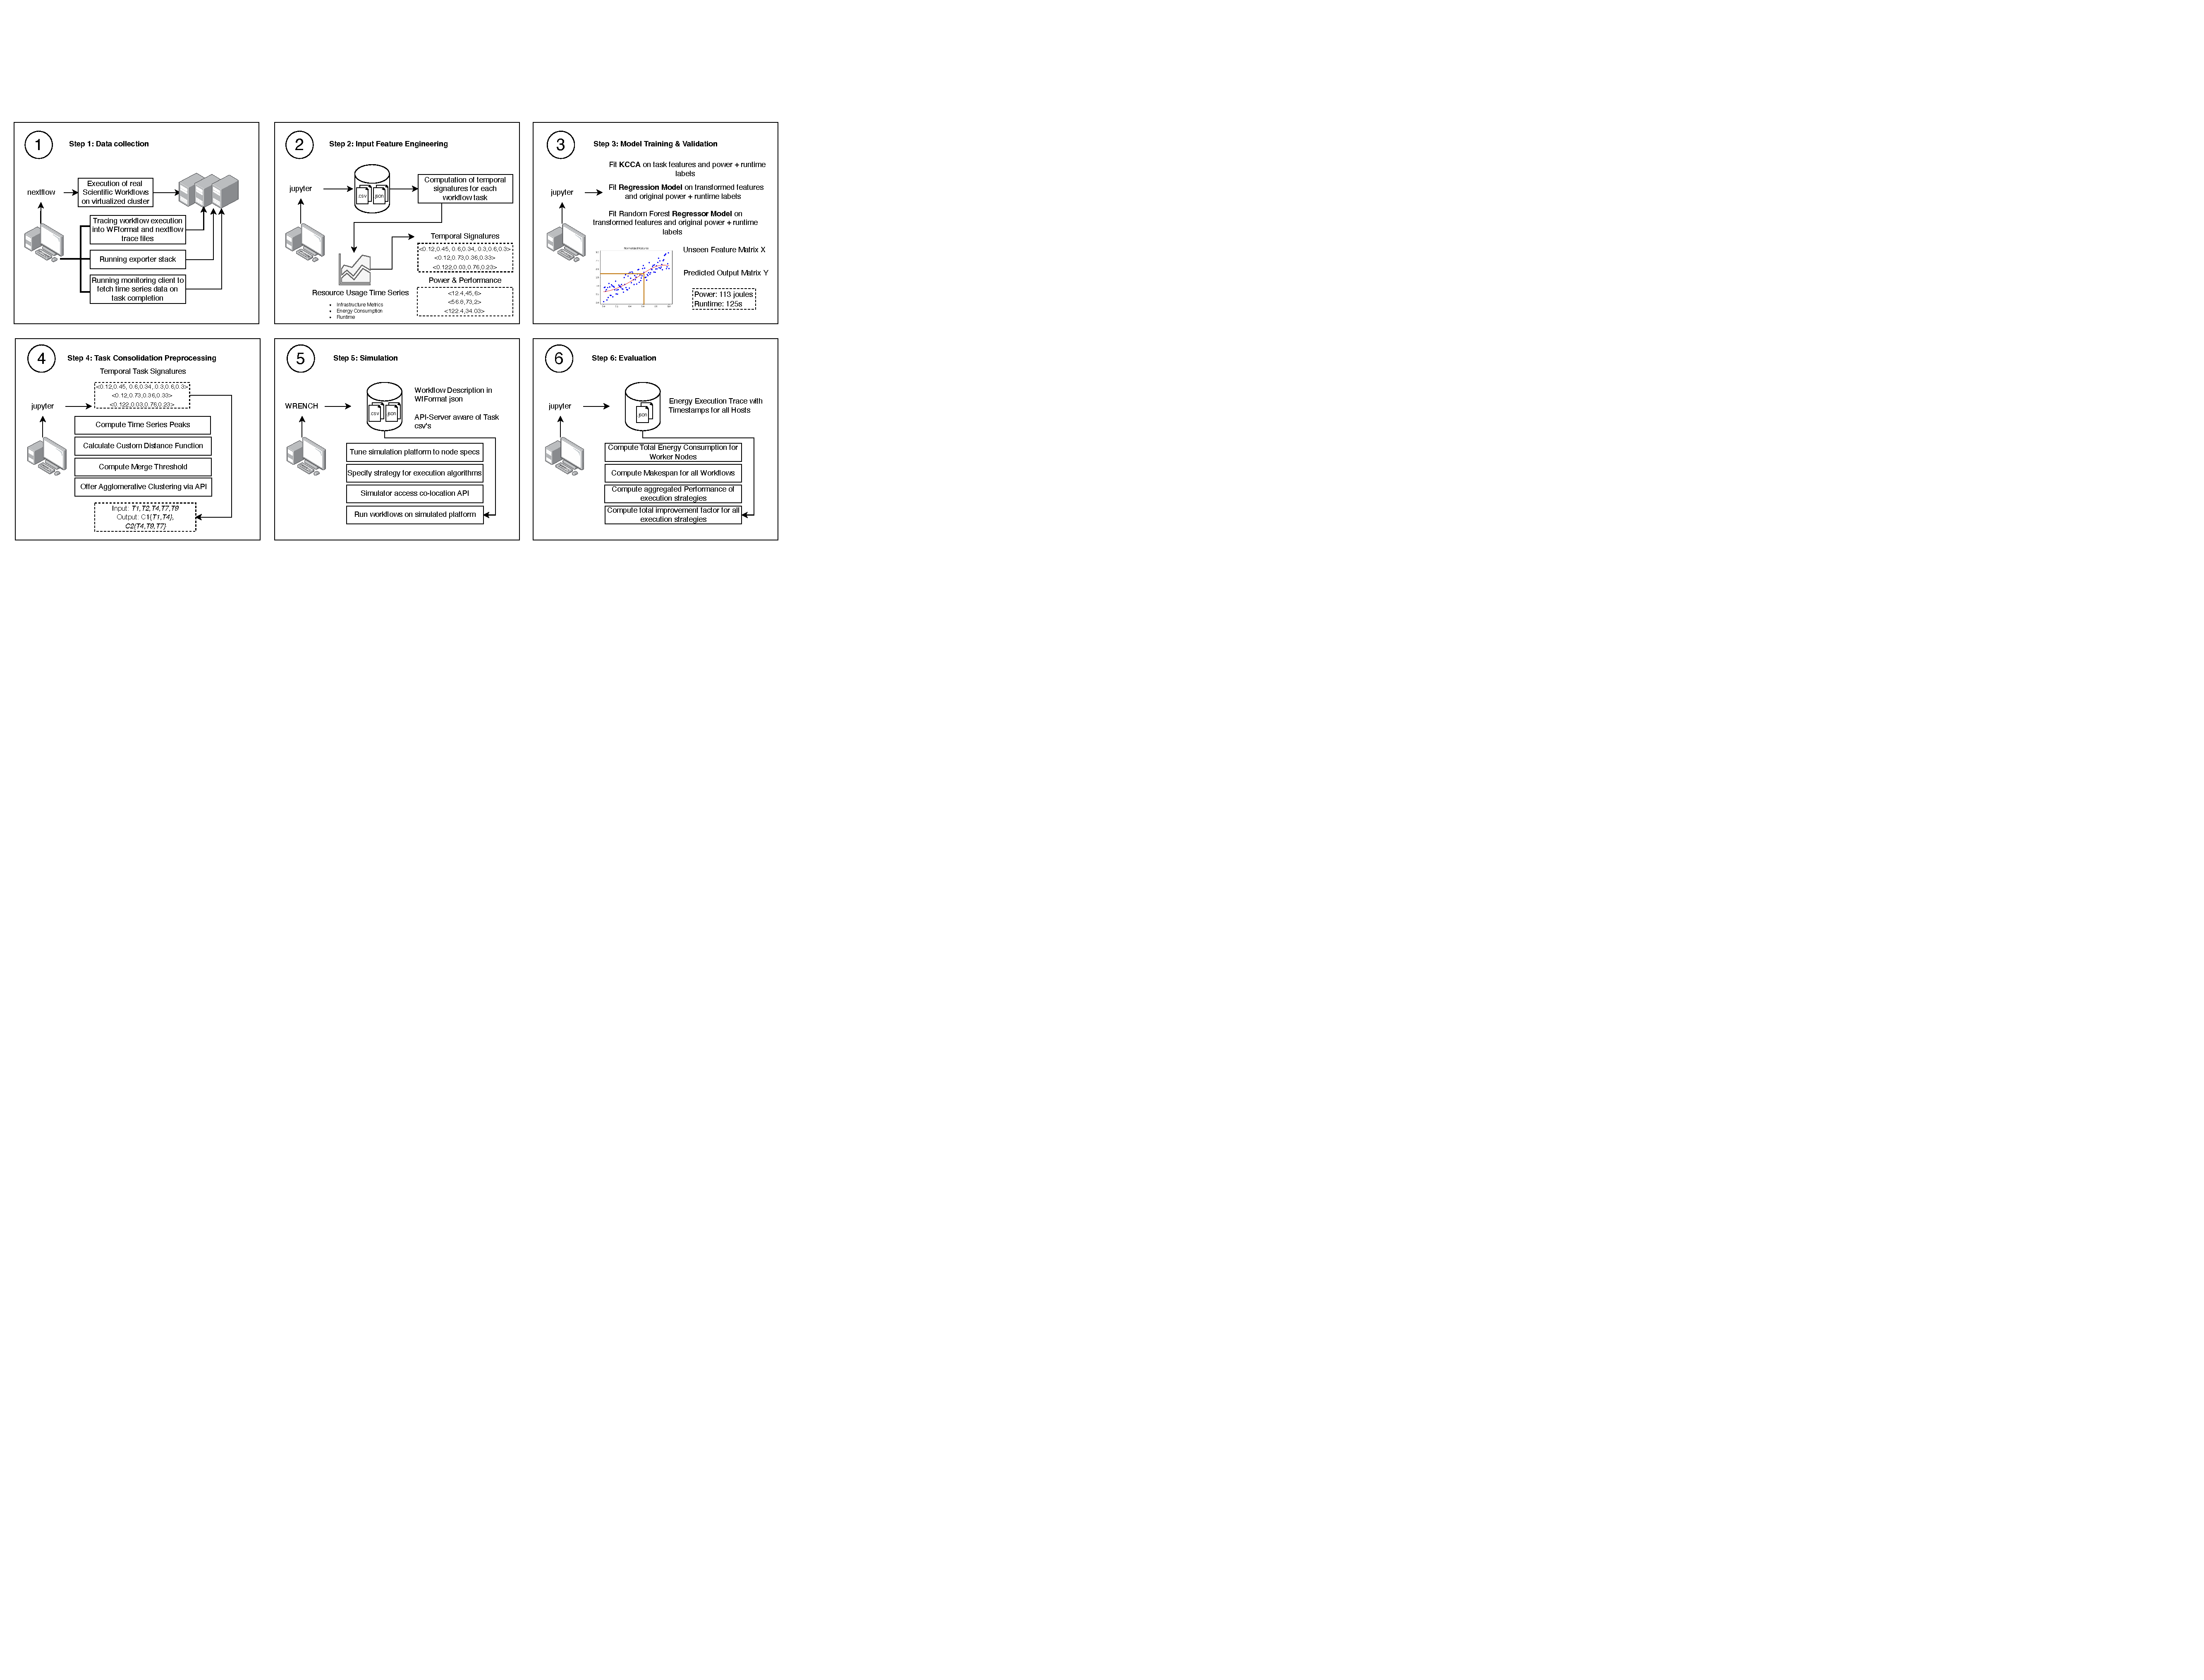
\includegraphics[width=\textwidth]{/home/nfomin3/dev/ThesisDocument/fig/04/04-overview.pdf} % Adjust the path if needed
    \caption{Overview of the approach consisting of 6 steps.}
    \label{fig:approach_overview}
\end{figure}

\subsection{Online Task Monitoring}
\label{sec:online_task_monitoring}

The online task monitoring approach builds on a hierarchical monitoring architecture that tries to captures a wide spectrum of metrics relevant to the execution of scientific workflows. The design is inspired by \cite{Bader_2022} targeting a four-layered structure consisting of the Resource Manager, Workflow, Machine, and Task layers. Each layer represents a distinct abstraction level in the workflow execution environment and provides valuable insights into different aspects of performance and resource utilization.

Starting with the Resource Manager layer a coarse-grained view related to cluster or partition status, resource allocation, and job management is provided. The Workflow layer operates on the logical workflow representation, maintaining execution progress, task dependencies, and overall runtime statistics. Below, the Machine layer captures system-level performance data such as CPU, memory, and storage utilization, as well as hardware-specific configurations. At the lowest level, the Task layer delivers fine-grained, time-resolved monitoring data, including per-task resource consumption, low-level kernel metrics, and execution traces.
\cite{Bader_2022}.

The following section provides a brief overview of the data sources and monitoring technologies that were ultimately assigned to the four layers of interest and thus selected for the approach. While the accompanying table presents a broader view of the different tools and data collection options that were tested the text below focuses only on the specific data sources that proved to be most reliable and effective within the implemented monitoring framework.

% TODO: Refine contents of the table here.
\begin{table}[htbp]
    \centering
    \setlength{\tabcolsep}{6pt} % adjust horizontal padding
    \renewcommand{\arraystretch}{1.2} % adjust vertical spacing
    \small % reduce overall text size to fit page
    \resizebox{\textwidth}{!}{
        \begin{tabular}{lccccccc}
            \toprule
            \textbf{Monitoring Features}        &
            \multicolumn{7}{c}{\textbf{Data Sources}}                                                                                                                                                                                  \\
            \cmidrule(lr){2-8}
                                                & \textbf{cAdvisor} & \textbf{ebpf-energy-exporter} & \textbf{docker-activity} & \textbf{scaphandre} & \textbf{slurm-exporter} & \textbf{process-exporter} & \textbf{cgroups-exporter} \\
            \midrule
            \multicolumn{8}{l}{\textbf{Resource Manager}}                                                                                                                                                                              \\[3pt]
            Infrastructure status               & x                 &                               &                          &                     &                         &                                                       \\
            File system status                  & x                 &                               &                          &                     &                         &                           &                           \\
            Running workflows                   & x                 &                               &                          &                     &                         &                           &                           \\
            \midrule
            \multicolumn{8}{l}{\textbf{Workflow}}                                                                                                                                                                                      \\[3pt]
            Status                              & x                 & x                             &                          &                     &                         &                           &                           \\
            Workflow specification              &                   & x                             &                          &                     &                         &                           &                           \\
            Graphical representation            &                   & x                             &                          &                     &                         &                           &                           \\
            Workflow ID                         & x                 & x                             &                          &                     &                         &                           &                           \\
            Execution report                    &                   & x                             &                          &                     &                         &                           &                           \\
            Previous executions                 &                   & x                             &                          &                     &                         &                           &                           \\
            \midrule
            \multicolumn{8}{l}{\textbf{Machine}}                                                                                                                                                                                       \\[3pt]
            Status                              &                   &                               & x                        & x                   &                         &                           &                           \\
            Machine type                        &                   &                               & x                        & x                   &                         &                           &                           \\
            Hardware specification              &                   &                               & x                        & x                   &                         &                           &                           \\
            Available resources                 &                   &                               & x                        & x                   &                         &                           &                           \\
            Used resources                      &                   &                               & x                        & x                   &                         &                           &                           \\
            \midrule
            \multicolumn{8}{l}{\textbf{Task}}                                                                                                                                                                                          \\[3pt]
            Task status                         &                   &                               &                          & x                   &                         &                           &                           \\
            Requested resources                 &                   &                               &                          & x                   &                         &                           &                           \\
            Consumed resources                  &                   &                               &                          & x                   &                         &                           &                           \\
            Resource consumption for code parts &                   &                               &                          & x                   &                         &                           &                           \\
            Task ID                             &                   &                               &                          & x                   &                         &                           &                           \\
            Application logs                    &                   &                               &                          & x                   &                         &                           &                           \\
            Task duration                       &                   &                               &                          & x                   &                         &                           &                           \\
            Low-level task metrics              &                   &                               &                          & x                   &                         &                           &                           \\
            Fault diagnosis                     &                   &                               &                          & x                   &                         &                           &                           \\
            \bottomrule
        \end{tabular}
    }
    \caption{Technologies and their capabilities evaluated against a 4-layered Monitoring Framework for Scientific Workflows.}
    \label{tab:monitoring-features}
\end{table}

Although monitoring plays a central role in enabling the presented methodology, the main objective of this thesis is not to evaluate the performance of monitoring tools or to develop new low-level monitoring frameworks for scientific workflows. Therefore, a detailed technical assessment of these tools is not provided here and will not be revisited in Chapter 6. Instead, a concise justification for the distinction between the tools that were experimentally explored and are shown in %\ref{tab:monitoring-features} and those that were finally chosen and used for actual data collection within the evaluation setup.

As shown in the %\ref{tab:monitoring-features}, the monitoring approach in this work was built around Prometheus as the chosen time-series database. Consequently, all monitoring tools were evaluated based on their interoperability with Prometheus, specifically their ability to function as exporters. The table lists the technologies that were examined for this purpose.

Since the main objective was to gain insight into workflow tasks executed as containers, the focus was on capturing detailed information at the container level and above. However, container-level data can sometimes result in non-identifiable entities, as container names may represent metadata that cannot be directly linked to specific workflow tasks or workflow instances. Therefore, the SMWS's built-in tracing capabilities remained valuable, as they provide a reliable mapping between workflow logic and system-level execution data.

Before describing the specific tools that were ultimately used for monitoring, it is important to briefly outline why certain exporters were excluded from further use. The Slurm exporter, a custom implementation, was originally intended to retrieve job-to-process mappings from the resource manager. However, equivalent information could also be obtained directly from the workflow engines tracing mechanism, and because Slurm's daemons introduced considerable overhead, the exporter was not used in later stages. The process exporter was also omitted due to difficulties in collecting and aggregating all process IDs associated with a single container. In many cases, only the initial shell process of a workflow task was captured, while its spawned subprocesses remained untracked.

Scaphandre, despite appearing promising at first, showed limited compatibility with AMD hardware, which was used in this work. It also struggled to capture short-lived tasks from the workflow management system, leading to incomplete datasets. Docker Activity, another RAPL-based exporter, performed reasonably well but was still constrained by its dependence on Intel power counters, which are only partially supported on AMD CPUs.

In the end, the most consistent and comprehensive results were achieved using cAdvisor and a custom eBPF-based exporter named ebpf-monitor, a modified fork of DEEP-mon \cite{8425477}. These two tools demonstrated the best stability and coverage across different task durations and resource types and were therefore selected for the final monitoring setup.

The following table presents the final selection of data sources that were retained for the monitoring setup, along with the specific metrics enabled for each source.
% TODO: Throw out the exporters that i did not end up using from the table.
% Table with Tool Overview and metrics
\begin{table}[htbp]
    \centering
    \setlength{\tabcolsep}{6pt}
    \renewcommand{\arraystretch}{1.2}
    \small
    \caption{Preliminary simulation results for a subset of workflows showing the overall improvement for both runtime and energy consumption compared to the average of 2 naive baselines without co-location.}
    \label{tab:workflow_results}
    % \resizebox{\textwidth}{!}{%
    \resizebox{\textwidth}{0.46\textheight}{%
        \begin{tabular}{
            >{\raggedright\arraybackslash}p{2.7cm}
            >{\raggedright\arraybackslash}p{3.3cm}
            >{\raggedright\arraybackslash}p{7cm}
            >{\raggedright\arraybackslash}p{2.7cm}
            }
            \toprule
            \textbf{Software Tool} & \textbf{Primary Focus}                                               & \textbf{Used Metrics}                                     & \textbf{Comment}                                                           \\
            \midrule
            nextflow               & Scientific Workflow Engine                                           & trace file summary                                        & Used for WfFormat generation and matching containers to nextflow processes \\
            \midrule
            cAdvisor               & Container Performance Monitor                                        & \makecell[l]{container\_memory\_working\_set\_bytes                                                                                    \\container\_memory\_usage\_bytes\\container\_memory\_rss\\container\_fs\_reads\_bytes\_total\\container\_fs\_writes\_bytes\_total\\container\_fs\_io\_current} & 11191 \\
            \midrule
            ebpf-monitor           & Container Energy \& Performance Monitor                              & \makecell[l]{container\_memory\_working\_set\_bytes                                                                                    \\container\_memory\_usage\_bytes\\container\_memory\_rss\\container\_fs\_reads\_bytes\_total\\container\_fs\_writes\_bytes\_total\\container\_fs\_io\_current\\container\_mem\_rss\\container\_mem\_pss\\container\_mem\_uss\\container\_kb\_r\\container\_kb\_w\\container\_num\_reads\\container\_disk\_avg\_lat\\container\_num\_writes\\container\_cycles\\container\_cpu\_usage\\container\_cache\_misses\\container\_cache\_refs\\container\_weighted\_cycles\\container\_power\\container\_instruction\_retired} & 39216.4 \\
            \midrule
            scaphandre             & Agent for electric power and energy consumption metrics              & \makecell[l]{scaph\_process\_disk\_total\_write\_bytes                                                                                 \\scaph\_process\_disk\_total\_read\_bytes\\scaph\_process\_memory\_virtual\_bytes\\scaph\_process\_memory\_bytes\\scaph\_process\_cpu\_usage\_percentage\\scaph\_process\_power\_consumption\_microwatts\\scaph\_process\_power\_consumption\_microwatts\\scaph\_host\_power\_microwatts\\scaph\_host\_energy\_microjoules} & 8257.7 \\
            \midrule
            docker-activity        & Monitoring Tool for container statistics and energy usage            & \makecell[l]{cpuEnergy                                                                                                                 \\cpuPercent\\cpuUsage\\memoryUsage} & 11191 \\
            \midrule
            process-exporter       & Prometheus exporter that mines /proc to report on selected processes & \makecell[l]{namedprocess\_namegroup\_cpu\_seconds\_total                                                                              \\namedprocess\_namegroup\_memory\_bytes\\namedprocess\_namegroup\_num\_threads\\namedprocess\_namegroup\_read\_bytes\_total\\namedprocess\_namegroup\_thread\_cpu\_seconds\_total\\namedprocess\_namegroup\_write\_bytes\_total} & 39216.4 \\
            \midrule
            slurm-exporter         & Slurm-based Exporter on Resource Management                          & (1/6) preliminary fastest co-location                     & 8257.7                                                                     \\
            \midrule
            cgroups-exporter       & Exporter for CGroups metrics, for LXD/Docker/systemd                 & \makecell[l]{cgroups\_memory\_pressure\_full\_total                                                                                    \\cgroups\_io\_pressure\_full\_total\\cgroups\_memory\_usage\\cgroups\_pids\_count\\cgroups\_cpu\_pressure\_full\_total} & 11191 \\
            \bottomrule
        \end{tabular}%
    }
\end{table}

% Description of cadvisor, ebpf-energy-monitor
cAdvisor is an open-source daemon for monitoring resource usage and performance of containers. It continuously discovers containers via Linux cgroups under the path /sys/fs/cgroup. Once started, cAdvisor subscribes to create/delete events in the cgroup filesystem, converts them to internal add/remove events, and configures per-container handlers. Metrics originate from machine-level facts parsed from /proc and /sys directories and most prominently container and process usage collected at cgroup boundaries. In practice, cAdvisor provides low-overhead, per-container telemetry.%\cite{Tol}.

The ebpf-monitor is based on the DEEP-Mon system, which is per-thread power attribution method to translate coarse-grained hardware power measurements into fine-grained, thread-level energy estimates by exploiting hardware performance counters. The Intel RAPL interface provides power readings per processor package or core, but it cannot distinguish how much of that energy was consumed by each thread. DEEP-Mon bridges this gap by observing how actively each thread uses the processor during each sampling interval. It does so by monitoring the number of unhalted core cycles—a counter that measures how long a core spends executing instructions rather than idling. Since power consumption correlates almost linearly with unhalted core cycles, the fraction of total cycles attributed to each thread provides a reasonable proxy for its share of energy usage.
In essence, DEEP-mon first computes the weighted cycles for each thread—combining its active cycles when alone with its proportionally reduced cycles when co-running. These weighted cycles determine how much of the total core-level RAPL energy should be assigned to that thread. The final per-thread power estimate is then derived by distributing the total measured power of each socket proportionally to the weighted cycle counts of all threads running on that socket. This approach allows DEEP-mon to infer realistic thread-level power usage even in systems with simultaneous multithreading and time-shared workloads, without modifying the scheduler or requiring any application-specific instrumentation. The DEEP-mon tool was modified in this work to export container-level metrics directly to Prometheus.

Based on this identification of relevant metrics and the according technologies, we now introduce the monitoring algorithm built on top of the selected exporter stack and the resulting overview of the needed components for implementing a suitable monitoring client that can efficiently behave like specified in %\ref{tab:monitoring_layers}. It outlines how these components were combined to realize the monitoring logic in this work, while the technical implementation details are described in %\ref{cha:implementation}.

First, we outline the core components that form the monitoring client and describe the strategy used to retrieve raw data from the monitored system.
\begin{figure}[htbp]
    \centering
    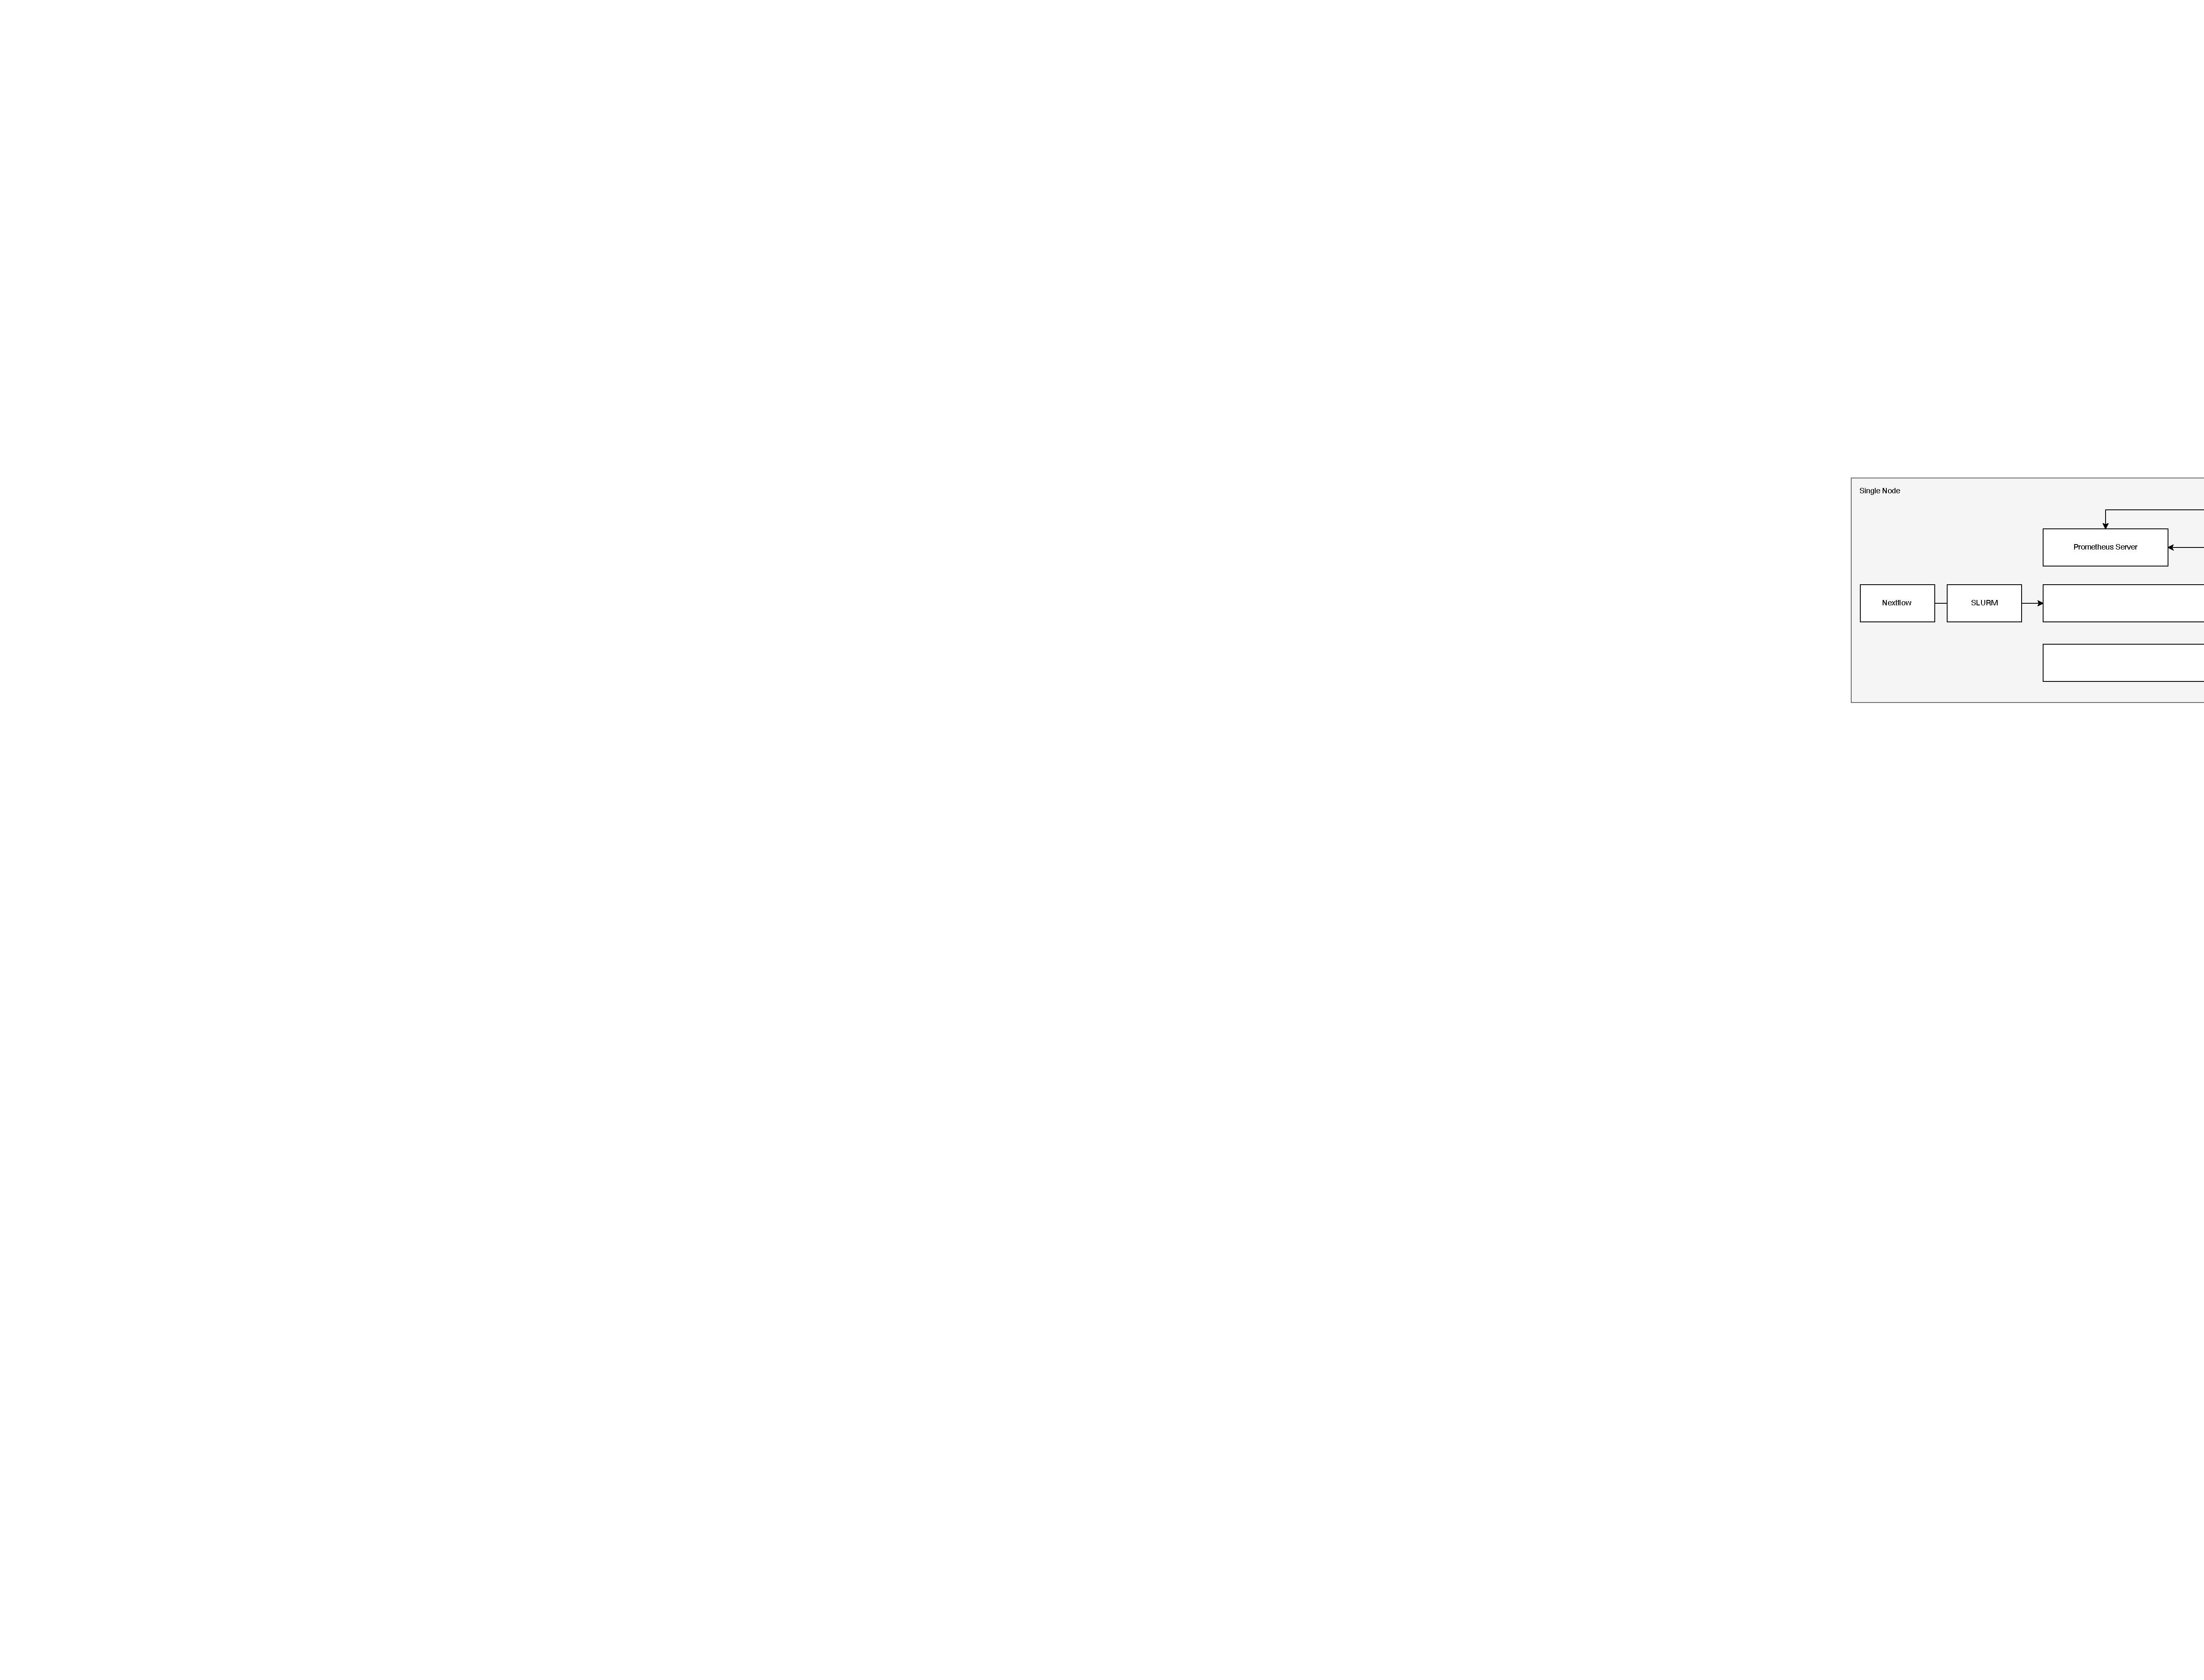
\includegraphics[width=\textwidth]{/home/nfomin3/dev/ThesisDocument/fig/04/04-monitoring.pdf} % Adjust the path if needed
    \caption{The monitoring client alongside the needed system components.}
    \label{fig:monitoring_client}
\end{figure}

%\ref{fig:monitoring_client} and \ref{alg:monitoring} show the principle behavior of the monitoring client. The event listener continuously observes container lifecycle events—such as start and termination—emitted by the runtime environment. Once an event is detected, the data query interface dynamically formulates PromQL queries based on the configuration and metadata of the affected container. These queries are sent to Prometheus to retrieve fine-grained time-series data. The retrieved raw metrics are then passed to the aggregation module, which aligns and consolidates them into a unified record per container.

% TODO: Add label here.
\begin{algorithm}[H]
    \caption{Event-Driven Monitoring and Metric Aggregation Framework}
    \label{alg:monitoring}
    \KwIn{Configuration $C$ defining monitoring targets}
    \KwOut{Aggregated container-level time-series metrics for each Nextflow process}

    \BlankLine
    initialize\_monitoring(C)\\
    init\_event\_listener()\\
    \While{true}{
        event $\gets$ wait\_for\_container\_event()\\
        meta $\gets$ extract\_metadata(event)\\
        \If{event.type = START}{
            register\_process(meta.id, meta.workflow\_label)
        }
        \If{event.type = TERMINATE}{
            metrics $\gets$ \{\}\\
            \ForEach{target $\in$ C.targets}{
                query $\gets$ build\_promql(target, meta.id, meta.time\_window)\\
                metrics[target] $\gets$ execute\_prometheus\_query(query)
            }
            data $\gets$ aggregate(metrics, meta.workflow\_label)\\
            store(data)
        }
    }
\end{algorithm}

% Algorithm Description
The design introduced in %\ref{alg:monitoring} reduces monitoring overhead and ensures that only relevant data are collected when workflow tasks actually execute. When a container start event is received, the client extracts metadata such as container ID, associated workflow label, and start timestamp, then registers the process in an internal mapping to maintain correspondence between container identifiers and workflow tasks. Upon receiving a termination event, the client triggers a targeted data collection phase. The monitoring client allows for dynamic configuration of the metrics mentioned in \ref{tab:monitoring-features}, enabling data analysis specifically scoped to the user's needs.

\subsection{Data Analysis}
\label{sec:data_analysis}
The next section describes the approach used to analyze the data collected through the monitoring client. The focus lies on how the raw metrics retrieved from Prometheus and other exporters were preprocessed, structured, and aligned to support both supervised and unsupervised learning tasks.

\subsubsection{Task Entity Matching}
\label{sec:task_entity_matching}
The first phase of the data analysis focuses on entity matching of heterogeneous monitoring data sources into a unified representation of each executed workflow task. During workflow execution, diverse monitoring tools and system components produce data at different abstraction levels.

% TODO: Add visualization of the data formats
The matching process begins with container lifecycle records, which provide information on task identifiers, container names, process hashes, and working directories. These files serve as the primary link between workflow-level entities and low-level monitoring data. Each monitoring source is traversed recursively to locate and load the associated time-series data. These data files are organized hierarchically under source-specific directories and often contain multiple interleaved measurements from different tasks. To facilitate task-level analysis, these aggregated time-series datasets need to be split into per-task CSV files.
Each per-task dataset is enriched with contextual metadata. The first enrichment phase attaches the correct working directory to every container trace, allowing file system references.
The next stage introduces workflow-level semantics by matching the per-task monitoring data with the workflows own metadata. Using the exported trace file by the SWMS, the analysis extracts task names and their corresponding working directories. These entries are matched against container-level records from the monitoring data to identify which monitored container corresponds to which logical task in the workflow. The resulting mapping is used to update all per-task monitoring files by appending the correct SWMS process name. This concludes the step of entity matching and preparing the collected data for further statistical analysis.

\subsection{Statistical Embedding and Learning}
\label{sec:statistical_embedding_and_learning}
\subsubsection{Data Preprocessing}
\label{sec:data_preprocessing}
% TODO: Add formal notation of the feature matrices
We transform the heterogeneous, time‐stamped monitoring traces into consistent task-level feature/label matrices suitable for statistical analysis. We therefore define the following preprocessing steps:

\begin{enumerate}
    \item Temporal signature construction (feature selection).
          \subitem Sampling and smoothing.
          \subitem Equal-length normalization.
          \subitem Container-wise collation.
    \item Model Input Construction.
          \subitem Normalization and Scaling.
          \subitem Extraction of Input Features and Output Labels.
\end{enumerate}

% Formal notation

\[
    \textbf{Temporal Signature and Model Input Construction.}
\]

We denote by \( \mathcal{T} = \{ T_1, T_2, \dots, T_N \} \) the set of
temporal signatures extracted from the monitored resource-usage profiles
of \( N \) workflow tasks.
Each task \( i \) is characterized by time-varying utilization traces
for the monitored resource dimensions
\[
    R = \{ \text{CPU}, \text{Memory}, \text{Disk}, \text{Network} \}.
\]

\noindent
For each resource \( r \in R \) and task \( i \),
the temporal signature \( T_i^{(r)} \) is defined as a
coarse-grained summary of the normalized resource usage signal
\( x_i^{(r)}(t) \):
\[
    T_i^{(r)} =
    \bigl\langle
    p_{1,i}^{(r)},\;
    p_{2,i}^{(r)},\;
    \dots,\;
    p_{10,i}^{(r)}
    \bigr\rangle,
    \tag{1}
\]
where each component \( p_{k,i}^{(r)} \) represents the mean
usage value within segment \( k \) of the time-normalized
execution window (\( k = 1, \dots, 10 \)).
This yields a ten-dimensional vector describing the temporal pattern of
resource consumption.

\noindent
The feature vector for task \( i \) is obtained by concatenating
the resource-specific signatures:
\[
    x_i =
    \bigl[
    T_i^{(\text{CPU})},\;
    T_i^{(\text{Memory})},\;
    T_i^{(\text{Disk})},\;
    T_i^{(\text{Network})}
    \bigr]
    \in \mathbb{R}^{d_x},
\]
where \( d_x = 4 \times 10 = 40 \) in this example configuration.

\[
    X =
    [x_1^\top, x_2^\top, \dots, x_N^\top]^\top
    \in \mathbb{R}^{N \times d_x}
\]
denotes the complete input matrix used for model training.

Similarly, for each task \( i \), the execution-level targets
(time and mean power consumption) are given by
\[
    y_i = [\,t_i,\, P_i\,] \in \mathbb{R}^2,
    \quad
    Y = [y_1^\top, y_2^\top, \dots, y_N^\top]^\top
    \in \mathbb{R}^{N \times 2}.
\]

\[
    \textbf{Example.}
\]
Consider \( N = 3 \) workflow tasks with simplified
CPU and memory usage signatures
(each consisting of 3 representative pattern points for brevity):
\[
    \begin{array}{lcccccc}
        \toprule
        \text{Task}        &
        p_1^{(\text{CPU})} & p_2^{(\text{CPU})} & p_3^{(\text{CPU})} &
        p_1^{(\text{Mem})} & p_2^{(\text{Mem})} & p_3^{(\text{Mem})}                             \\
        \midrule
        1                  & 0.40               & 0.75               & 0.90 & 0.35 & 0.55 & 0.60 \\
        2                  & 0.20               & 0.50               & 0.70 & 0.25 & 0.40 & 0.50 \\
        3                  & 0.30               & 0.65               & 0.85 & 0.30 & 0.45 & 0.55 \\
        \bottomrule
    \end{array}
\]

Concatenating these signatures yields the input matrix
\[
    X =
    \begin{bmatrix}
        0.40 & 0.75 & 0.90 & 0.35 & 0.55 & 0.60 \\
        0.20 & 0.50 & 0.70 & 0.25 & 0.40 & 0.50 \\
        0.30 & 0.65 & 0.85 & 0.30 & 0.45 & 0.55
    \end{bmatrix},
    \quad
    Y =
    \begin{bmatrix}
        12.4 & 65 \\
        14.1 & 72 \\
        10.8 & 58
    \end{bmatrix}.
\]

Here, each row of \( X \) encodes the temporal resource-usage pattern
of a task, while \( Y \) provides the corresponding runtime and mean
power consumption used for model learning or correlation analysis.

This preprocessing yields: (i) a standardized and fixed-length feature matrix X that preserves per-metric usage distributions and (ii) a label matrix Y capturing runtime and energy

\subsubsection{Predictive Modeling}
\label{sec:predictive_modeling}

% Add intro sentence why we are doing that.

In the next step of the analysis, the collected and preprocessed task data are prepared for statistical learning. The objective is to identify relationships between task-specific features and their corresponding performance and energy characteristics. To achieve this, the dataset is divided into two parts: approximately 70\% of the tasks are used for training the models, while the remaining 30\% are reserved for testing and validation.

Before training, both the feature data (X) and the target data (Y)—representing task runtime and energy consumption—are standardized separately. Each is transformed to have a mean of zero and a standard deviation of one. This step is essential, as the original values cover different numerical scales, which could negatively affect kernel-based learning methods. Standardization ensures that all features contribute equally to the learning process and prevents those with larger magnitudes from biasing the results.

\paragraph{Kernel Canonical Correlation Analysis (KCCA)}
\label{sec:kcca}
After normalization, a Kernel Canonical Correlation Analysis (KCCA) model is trained to identify shared patterns between the feature data and the target data. KCCA projects both datasets into a common latent space, where it can detect nonlinear relationships between resource usage patterns and their corresponding runtime and energy behavior.

Once trained, the KCCA model is extended into a predictive framework. The latent features learned from the input data are used to fit a regression model that links these representations to runtime and energy targets. This allows the system not only to capture statistical relationships but also to predict performance and energy consumption for unseen tasks.

% Notation
\[
    \textbf{Kernel Canonical Correlation Analysis (KCCA).}
\]
To capture nonlinear dependencies between the resource signatures
and performance power outcomes, we apply Gaussian kernels to both
input and output feature spaces.

KCCA seeks directions \(A\) and \(B\) in the
reproducing kernel spaces of \(K_x\) and \(K_y\)
that maximize the correlation between
\( K_x A \) and \( K_y B \).
This is expressed as the generalized eigenvalue problem:
\[
    \begin{bmatrix}
        0       & K_y K_x \\
        K_x K_y & 0
    \end{bmatrix}
    \begin{bmatrix}
        A \\ B
    \end{bmatrix}
    =
    \lambda
    \begin{bmatrix}
        K_x^2 & 0     \\
        0     & K_y^2
    \end{bmatrix}
    \begin{bmatrix}
        A \\ B
    \end{bmatrix}.
    \tag{2}
\]

Solving (2) yields paired canonical directions
\( (A, B) \) that define latent projections
\[
    X' = K_x A, \qquad Y' = K_y B,
\]
maximally correlated across the two feature spaces.
These projections represent a shared latent space
relating resource utilization dynamics to task performance and energy.

\[
    \textbf{Illustrative Example.}
\]
Consider three workflow tasks \( i = 1, 2, 3 \)
with aggregated temporal signatures over CPU and memory:
\[
    x_1 = [0.40,\, 0.75,\, 0.90,\, 0.35,\, 0.55,\, 0.60], \quad
    x_2 = [0.20,\, 0.50,\, 0.70,\, 0.25,\, 0.40,\, 0.50], \quad
    x_3 = [0.30,\, 0.65,\, 0.85,\, 0.30,\, 0.45,\, 0.55].
\]
Their corresponding runtime power outcomes are:
\[
    y_1 = [12.4,\, 65], \quad
    y_2 = [14.1,\, 72], \quad
    y_3 = [10.8,\, 58].
\]

KCCA maps both the temporal patterns \(x_i\)
and the performance power pairs \(y_i\)
into high-dimensional kernel spaces
and finds projections that maximize their mutual correlation.
In this example, the first canonical mode reveals that
tasks with higher sustained CPU activity
(\(x_1, x_3\))
correspond to lower execution time and reduced power consumption,
while the less efficient task (\(x_2\))
shows a distinct temporal signature characterized by
fluctuating utilization and higher runtime.

\paragraph{Random Forest Regression}
\label{sec:random_forest_regression}
To complement the KCCA model, we trained two non-parametric regressors based on Random Forests—one to predict mean task power and one to predict task runtime from the same preprocessed feature matrix. The power model is trained on mean per-task energy-rate labels, while the runtime model uses task durations as targets. As a sanity check, we established simple baselines by predicting the training-set mean once for power and once for runtime on the test split. These baselines quantify the minimum improvement any learned model must exceed.

\subsection{Unsupervised Learning}
\label{sec:unsupervised_learning}
% Add intro sentence why we are doing that.
Using the temporal signature feature representation of the monitored tasks, we establish the basis for energy-aware task co-location. Co-location is treated as a consolidation problem, formulated through a clustering approach. In this context, clustering groups tasks based on a defined distance measure that captures their similarity. To incorporate energy awareness into this objective we extend the distance definition to account for interference between workloads. This is achieved by conducting separate workload experiments designed to measure resource contention and interaction effects. From these experiments, affinity scores are derived to quantify how different workloads influence each other when co-located. These affinity scores are then integrated into the clustering distance function, ensuring that both performance and energy interactions guide the co-location decisions.

\subsubsection{Measuring Resource Contention}
\label{sec:measuring_resource_contention}

The measurement of resource contention follows a two-stage protocol that first establishes isolated baselines for each workload class and then repeats the same workloads under controlled co-location. In the baseline stage, CPU-bound, memory-bound, and file-I/O-bound containers are executed one at a time on pinned logical CPUs. Pinning fixes placement and removes scheduler noise; for I/O experiments the file set is prepared once and cleaned afterward to avoid warm-cache artifacts. Each run records a start and finish timestamp at microsecond resolution and derives the wall-clock duration. In parallel, the monitoring pipeline supplies per-container power time series. After a run finishes, only the power streams belonging to the participating container are retained, aligned to the containers lifetime, and summarized to a representative mean value.
The co-location stage replays the same workloads in pairs to expose interference effects. Pairs are chosen to cover both homogeneous combinations, where both containers stress the same resource class, and heterogeneous combinations, where their dominant pressure differs. Placement again uses CPU pinning. Some experiments bind pairs to siblings on the same physical core to amplify shared-core effects; others place them on distinct cores to isolate memory bandwidth or storage contention. Each co-located container is measured in exactly the same way as in isolation, producing a matched set of durations and power summaries.

% Table for the experiment design


\begin{table}[htbp]
    \centering
    \caption{Summary of Synthetic Benchmarks Used in Evaluation}
    \label{tab:synthetic-benchmarks}
    \begin{tabular}{@{}lcccc@{}}
        \toprule
        \textbf{Benchmark Label}                                                                                                                          & \textbf{Image / Version} & \textbf{Execution Command} & \textbf{Behavior Type} & \textbf{Comments} \\
        \midrule

        \textbf{CPU}                                                                                                                                      &
        \texttt{stress-ng-cpu:latest}                                                                                                                     &
        \texttt{stress-ng --cpu 1 --cpu-method matrixprod --cpu-ops 100000 --metrics-brief}                                                               &
        CPU-bound, matrix computation kernel.                                                                                                             &
        Used to emulate high arithmetic intensity workloads.                                                                                                                                                                                                   \\

        \textbf{Memory (VM)}                                                                                                                              &
        \texttt{stress-ng-mem-vm:latest}                                                                                                                  &
        \texttt{stress-ng --vm 1 --vm-bytes 18G --vm-ops 1000 --metrics-brief}                                                                            &
        Memory-bound workload.                                                                                                                            &
        Tests VM allocation, memory contention, and NUMA effects.                                                                                                                                                                                              \\

        \textbf{File I/O}                                                                                                                                 &
        \texttt{fio:latest}                                                                                                                               &
        \texttt{fio --name seqread --rw read --bs 1M --size 18G --numjobs 1 --readonly=1 --direct=1 --iodepth=32 --ioengine=io\_uring --group\_reporting} &
        I/O-intensive sequential read.                                                                                                                    &
        Evaluates disk and I/O scheduling performance.                                                                                                                                                                                                         \\
        \bottomrule
    \end{tabular}
\end{table}

% Notation for the experiments.
\[
    \textbf{Isolated and Co-located Metrics.}
\]

For each workload \( i \in \{1,2\} \), let
\[
    t_i^{(iso)}, \; t_i^{(coloc)} \quad \text{denote the isolated and co-located runtimes,}
\]
\[
    P_i^{(iso)}, \; P_i^{(coloc)} \quad \text{denote the average isolated and co-located power consumption.}
\]

\[
    \textbf{Per-workload Slowdown Factors.}
\]

For each workload \( i \in \{1, 2\} \), let
\[
    t_i^{(iso)}, \; t_i^{(coloc)} \quad \text{denote isolated and co-located runtimes,}
\]
\[
    P_i^{(iso)}, \; P_i^{(coloc)} \quad \text{denote isolated and co-located average power consumptions.}
\]

The per-workload slowdowns are defined as
\[
    S_i^{(t)} = \frac{t_i^{(coloc)}}{t_i^{(iso)}},
    \qquad
    S_i^{(P)} = 1 + \log\!\left(
    \max\!\left( \frac{P_i^{(coloc)}}{P_i^{(iso)}}, 1 \right)
    \right),
\]
ensuring that both runtime and power slowdowns are
non-negative and at least one in value.

The mean slowdowns across the workload pair are
\[
    \bar{S}^{(t)} = \frac{S_1^{(t)} + S_2^{(t)}}{2},
    \qquad
    \bar{S}^{(P)} = \frac{S_1^{(P)} + S_2^{(P)}}{2}.
\]

A weighted average combines both effects:
\[
    \bar{S} =
    \alpha\, \bar{S}^{(t)} + (1 - \alpha)\, \bar{S}^{(P)},
    \quad \text{with } \alpha \in [0,1],
\]
where higher \(\alpha\) emphasizes runtime effects,
and lower \(\alpha\) gives more weight to power efficiency.

The final combined slowdown factor is
\[
    \bar{S}_{\text{final}} = \max(1, \bar{S}),
\]
guaranteeing that co-location never yields an apparent
speedup (values \(\ge 1\) indicate slowdown).

\[
    \textbf{Affinity Score.}
\]

The affinity score \(A\) quantifies the degree of
interference between two co-located workloads.

First, compute pairwise affinity ratios:
\[
    A^{(t)} =
    \frac{t_1^{(coloc)} + t_2^{(coloc)}}
    {t_1^{(iso)} + t_2^{(iso)}},
    \qquad
    A^{(P)} =
    1 + \log\!\left(
    \max\!\left(
    \frac{P_1^{(coloc)} + P_2^{(coloc)}}
    {P_1^{(iso)} + P_2^{(iso)}},
    1
    \right)
    \right).
\]

A weighted average combines both effects:
\[
    A_{\text{raw}} =
    \alpha\, A^{(t)} + (1 - \alpha)\, A^{(P)},
    \qquad A_{\text{raw}} \ge 1.
\]

The normalized affinity score is then:
\[
    A =
    \frac{1 - \frac{1}{A_{\text{raw}}}}{\beta},
    \qquad A \in [0, 1],
\]
where \(\beta > 0\) controls scaling sensitivity.
Values of $A \approx 0$ indicate minimal interference,
while \(A \to 1\) signifies strong co-location interference.

% TODO: Write that this yields in an affinity score matrix and insert example.
% TODO: Reference the table with some explanations.

\begin{table}[H]
    \centering
    \caption{Affinity scores between workload types indicating co-location compatibility.}
    \label{tab:affinity_scores}
    \begin{tabularx}{\textwidth}{l l c X}
        \toprule
        \textbf{Workload 1} & \textbf{Workload 2} & \textbf{Affinity Score} & \textbf{Comment}                                                                              \\
        \midrule
        mem                 & cpu                 & 0.543                   & Moderate compatibility; memory and CPU workloads can share resources with limited contention. \\
        mem                 & fileio              & 0.148                   & Very low compatibility; strong interference due to I/O and memory bandwidth pressure.         \\
        fileio              & cpu                 & 0.223                   & Low compatibility; CPU workloads cause contention for shared I/O buffers.                     \\
        cpu                 & cpu                 & 0.444                   & Medium self-affinity; CPU-bound tasks compete for cores but remain schedulable.               \\
        mem                 & mem                 & 0.514                   & Moderate self-affinity; memory contention manageable under shared caching.                    \\
        fileio              & fileio              & 0.346                   & Limited self-affinity; file I/O contention degrades throughput under co-location.             \\
        \bottomrule
    \end{tabularx}
\end{table}

From these measurements, contention is characterized by comparing the co-located outcomes against the isolated baselines for the same workloads. For each pair, the procedure derives how much slower the workloads ran together relative to alone and how their average power changed. To avoid overfitting to any single signal, runtime and power effects are aggregated into a single scalar that captures the overall quality of the pairing. Values above a neutral threshold indicate that the pair plays well together, while values below it signal destructive interference. This single number is what the co-location policies use downstream: it serves both as the supervision signal for learning-based components and as the ground truth to validate scheduling heuristics in simulation.

\subsubsection{Task Clustering}
\label{sec:task_clustering}
Consolidation is formulated as a clustering problem with an important modification: rather than grouping tasks that are similar, the goal is to cluster tasks with complementary resource usage patterns to minimize contention during co-location. Building on the previously established notion of affinity—which quantifies how strongly workloads interfere when sharing resources—the clustering process now incorporates this measure directly into its distance metric. The task task distance increases when two tasks exert pressure on the same resources simultaneously, indicating potential contention, and decreases when their resource usage peaks complement one another.
Algorithm %\ref{alg:task_distance_clustering} summarizes the main stages of the task consolidation procedure used in this work. The approach begins by computing pairwise similarities between task signatures, where each signature represents a multi-dimensional profile of resource usage over time. The similarity computation incorporates resource affinity weights derived from the contention experiments, ensuring that tasks are compared not only by magnitude but also by their impact on shared resources such as CPU, memory, and I/O. This yields a resource-aware similarity matrix that reflects how well tasks can coexist on the same node without interference.
Next, a percentile-based threshold is applied to the similarity matrix. This adaptive rule determines when clustering should stop by selecting only the most suitable task pairs according to the defined percentile. In this way, the algorithm avoids arbitrary distance cutoffs and instead adapts to the underlying distribution of similarity values.
Finally, agglomerative clustering is performed using a specified linkage criterion, such as average or complete linkage, to iteratively merge tasks into clusters. Each resulting cluster represents a potential consolidation group, meaning a set of tasks that can be executed together within a single virtual machine due to complementary or non-overlapping resource demands. The output clusters thus provide a structured view of optimal co-location candidates for subsequent scheduling and energy-aware execution strategies.

% Algorithm for Task Consolidation in ShaReComp
\begin{algorithm}[H]
    \caption{ShaReComp - Task Consolidation Algorithm}
    \label{alg:task_distance_clustering}
    \SetKwFunction{Sim}{compute\_similarity}
    \SetKwFunction{Thresh}{percentile\_threshold}
    \SetKwFunction{Merge}{agglomerative\_merge}

    \KwIn{task signatures $\mathrm{sig}$, affinity weights $w$, percentile $\tau$, linkage}
    \KwOut{clusters $\mathcal{C}$}

    $S \gets$ \Sim($\mathrm{sig}$, $w$) \tcp*[r]{resource-aware similarity}
    $\theta \gets$ \Thresh($S$, $\tau$) \tcp*[r]{percentile-based stopping rule}
    $\mathcal{C} \gets$ \Merge($S$, $\theta$, linkage) \tcp*[r]{agglomerative clustering}

    \textbf{return } $\mathcal{C}$
\end{algorithm}

Next, we introduce the subsequent steps necessary to fullfill %\ref{alg:task_distance_clustering}, focusing on how the task data needs to be refined.

\begin{enumerate}
    \item Peak-pattern construction. For every task and monitored workload type, we first derive a peak time series: the raw per-second resource signal is resampled into three-second buckets and the maximum per bucket is retained. When two peak series must be compared, we truncate both to the shorter length so that correlation is computed on aligned vectors without padding artifacts.
    \item Workload-type affinity. Different resource domains interfere to different degrees such as CPU vs CPU peaks are typically more contentious than CPU vs file I/O. We encode this with an empirical affinity score defined in the prior section between workload types. High affinity means higher potential interference when peaks align; low affinity reflects benign coexistence.
    \item Anti-similarity distance. For any pair of tasks i,j, we iterate over their workload types and compute two ingredients: (i) the affinity between the two types; (ii) the correlation between their corresponding peak series computed twice, once per type, to capture both sides of the pairing. We then aggregate these terms so that highly correlated peaks in high-affinity domains increase the distance, whereas low or negative correlations in low-affinity pairs decrease it. The result is a symmetric task distance matrix whose off-diagonal entries quantify how bad it would be to co-locate the two tasks, and whose diagonals are zero by definition.

          % Notation for the distance formula
          \[
              \textbf{Inter-Task Distance and Resource Correlation Model}
          \]

          To quantify the similarity and potential contention between two workloads
          \( i \) and \( j \), we define a composite distance measure
          that integrates both resource affinity and correlation of peak usage.
          Each workload utilizes a set of resources
          \( R = \{ \text{CPU}, \text{Memory}, \text{Disk}\} \),
          yielding in total ten pairwise combinations of resource types across two tasks.
          The distance term combines the precomputed affinity score with the
          correlation of peak resource intensities.

          \[
              D_{i,j}
              = \sum_{R_1, R_2}
              \Bigl(
              (\mathrm{aff\text{-}score}(R_1^i, R_2^j))
              \cdot
              \mathrm{Corr}(\mathrm{peak}\,R_1^i, \mathrm{peak}\,R_1^j)
              \cdot
              \mathrm{Corr}(\mathrm{peak}\,R_2^i, \mathrm{peak}\,R_2^j)
              \Bigr)
              \tag{1}
          \]

          where:
          \begin{align}
              R_1^i, R_2^j & \; \text{denote resource types of workloads } i \text{ and } j,                           \\[4pt]
              \mathrm{Corr}(\mathrm{peak}\,R_1^i, \mathrm{peak}\,R_1^j)
                           & \; \text{is the Pearson correlation between the peak usages of resource } R_1,            \\[4pt]
              \mathrm{aff\text{-}score}(R_1^i, R_2^j)
                           & \in [0, 1] \text{ measures the degree of interference between } R_1^i \text{ and } R_2^j.
          \end{align}

          \[
              \textbf{Interpretation}
          \]

          The intuition behind this distance metric is to
          \emph{promote dissimilar task pairings} for co-location.
          If two workloads exhibit highly correlated peak usage on the same resources,
          their corresponding correlation terms will be large,
          thus increasing \( D_{i,j} \) and discouraging their co-location.
          Conversely, tasks with uncorrelated or complementary resource peaks
          yield smaller distance values and are therefore more suitable to merge.

          The affinity score modulates this behavior:
          smaller values of \( \mathrm{aff\text{-}score} \)
          indicate lower interference between resource pairs,
          which can offset strong peak correlations.

          Finally, clustering proceeds by iteratively merging task clusters
          whose inter-cluster distance satisfies:
          \[
              D_{i,j} < \text{merge\_threshold}.
          \]
          This ensures that only compatible workloads, in terms of both
          resource affinity and temporal peak correlation, are grouped together.
    \item \textbf{Threshold selection}. Because the distance matrix is data-dependent, we estimate a merge threshold directly from its empirical distribution. A quantile for e.g., the 20th percentile on the raw distances acts as an automatic cut-level: any pair below this threshold is safe enough to consider for co-location, while pairs above it are kept apart.
    \item \textbf{Agglomerative clustering with precomputed distances}. We run average-linkage agglomerative clustering on the precomputed distance matrix with the chosen distance threshold and no preset cluster count. This yields variable-sized clusters whose members are mutually non-contentious under our metric. Because we use a threshold rather than a fixed k, the method adapts to each workload mix, producing more or fewer groups as warranted by the observed interference structure.
    \item\textbf{From clusters to co-location candidates}. Each cluster defines a candidate co-location set. To make these cluster-level entities usable by predictive models such as introduced in %\ref{sec:statistical_embedding_and_learning}, we construct cluster feature vectors by flattening and concatenating the per-task temporal signatures of all members and summing them dimension-wise. This potentially approximates the combined load shape we would see if the clusters tasks were executed in a co-located manner.
\end{enumerate}

\subsection{Combining supervised and unsupervised learning}
\label{sec:combining_supervised_and_unsupervised_learning}

% Algorithm for prediction of task clusters.
\begin{algorithm}[H]
    \caption{ShaReComp — Prediction of Energy and Performance Behavior of Consolidated Task Clusters}
    \label{alg:sharecomp_prediction}
    \SetKwFunction{Aggregate}{sum\_cluster\_features}
    \SetKwFunction{Build}{build\_feature\_matrix}
    \SetKwFunction{Predict}{predict\_runtime\_and\_energy}

    \KwIn{task clusters $\mathcal{C}$, per-task signatures $\mathrm{sig}$, trained model $\mathcal{M}$ (KCCA or Random Forest)}
    \KwOut{predicted runtime energy pairs $\hat{Y} = \{ (\hat{t}_k, \hat{E}_k) \}$}

    \BlankLine
    \ForEach{cluster $C_k \in \mathcal{C}$}{
        $F_k \gets$ \Aggregate($\{\,\mathrm{sig}[t_i] \mid t_i \in C_k\,\}$) \tcp*[r]{sum task signatures to form cluster feature}
    }
    $X \gets$ \Build($\{F_k\}$) \tcp*[r]{construct consolidated feature matrix}

    \BlankLine
    \ForEach{cluster feature $X_k \in X$}{
        $(\hat{t}_k, \hat{E}_k) \gets$ \Predict($X_k$, $\mathcal{M}$)
    }
    \BlankLine
    \textbf{return } $\hat{Y} = \{ (\hat{t}_k, \hat{E}_k) \}_{k=1}^{|\mathcal{C}|}$
\end{algorithm}

% Example on how this looks
\textbf{Example.}
Assume two clusters:
\[
    C_1 = \{t_1, t_2\}, \quad C_2 = \{t_3\},
\]
and each task has a CPU Memory signature with three pattern points:
\[
    t_1 = [0.4, 0.7, 0.9, 0.5, 0.6, 0.7], \quad
    t_2 = [0.3, 0.5, 0.8, 0.4, 0.5, 0.6], \quad
    t_3 = [0.2, 0.4, 0.6, 0.3, 0.4, 0.5].
\]
Cluster features are summed:
\[
    F_1 = t_1 + t_2 = [0.7, 1.2, 1.7, 0.9, 1.1, 1.3], \quad
    F_2 = t_3.
\]
Model predictions yield
\[
    \hat{Y} =
    \begin{bmatrix}
        10.8 & 62.5 \\
        14.2 & 75.1
    \end{bmatrix},
\]
representing predicted runtime (s) and energy (W) per cluster.

\subsection{Simulation Environment}
\label{sec:simulation_environment}

\subsubsection{Design Pillars}
\label{sec:design_pillars}


The simulator for co-location strategies builds upon three fundamental design pillars that reflect the main optimization opportunities identified in the co-location problem: resource allocation, queue ordering, and job placement.

% Figure with Simulator Design
\begin{figure}[htbp]
    \centering
    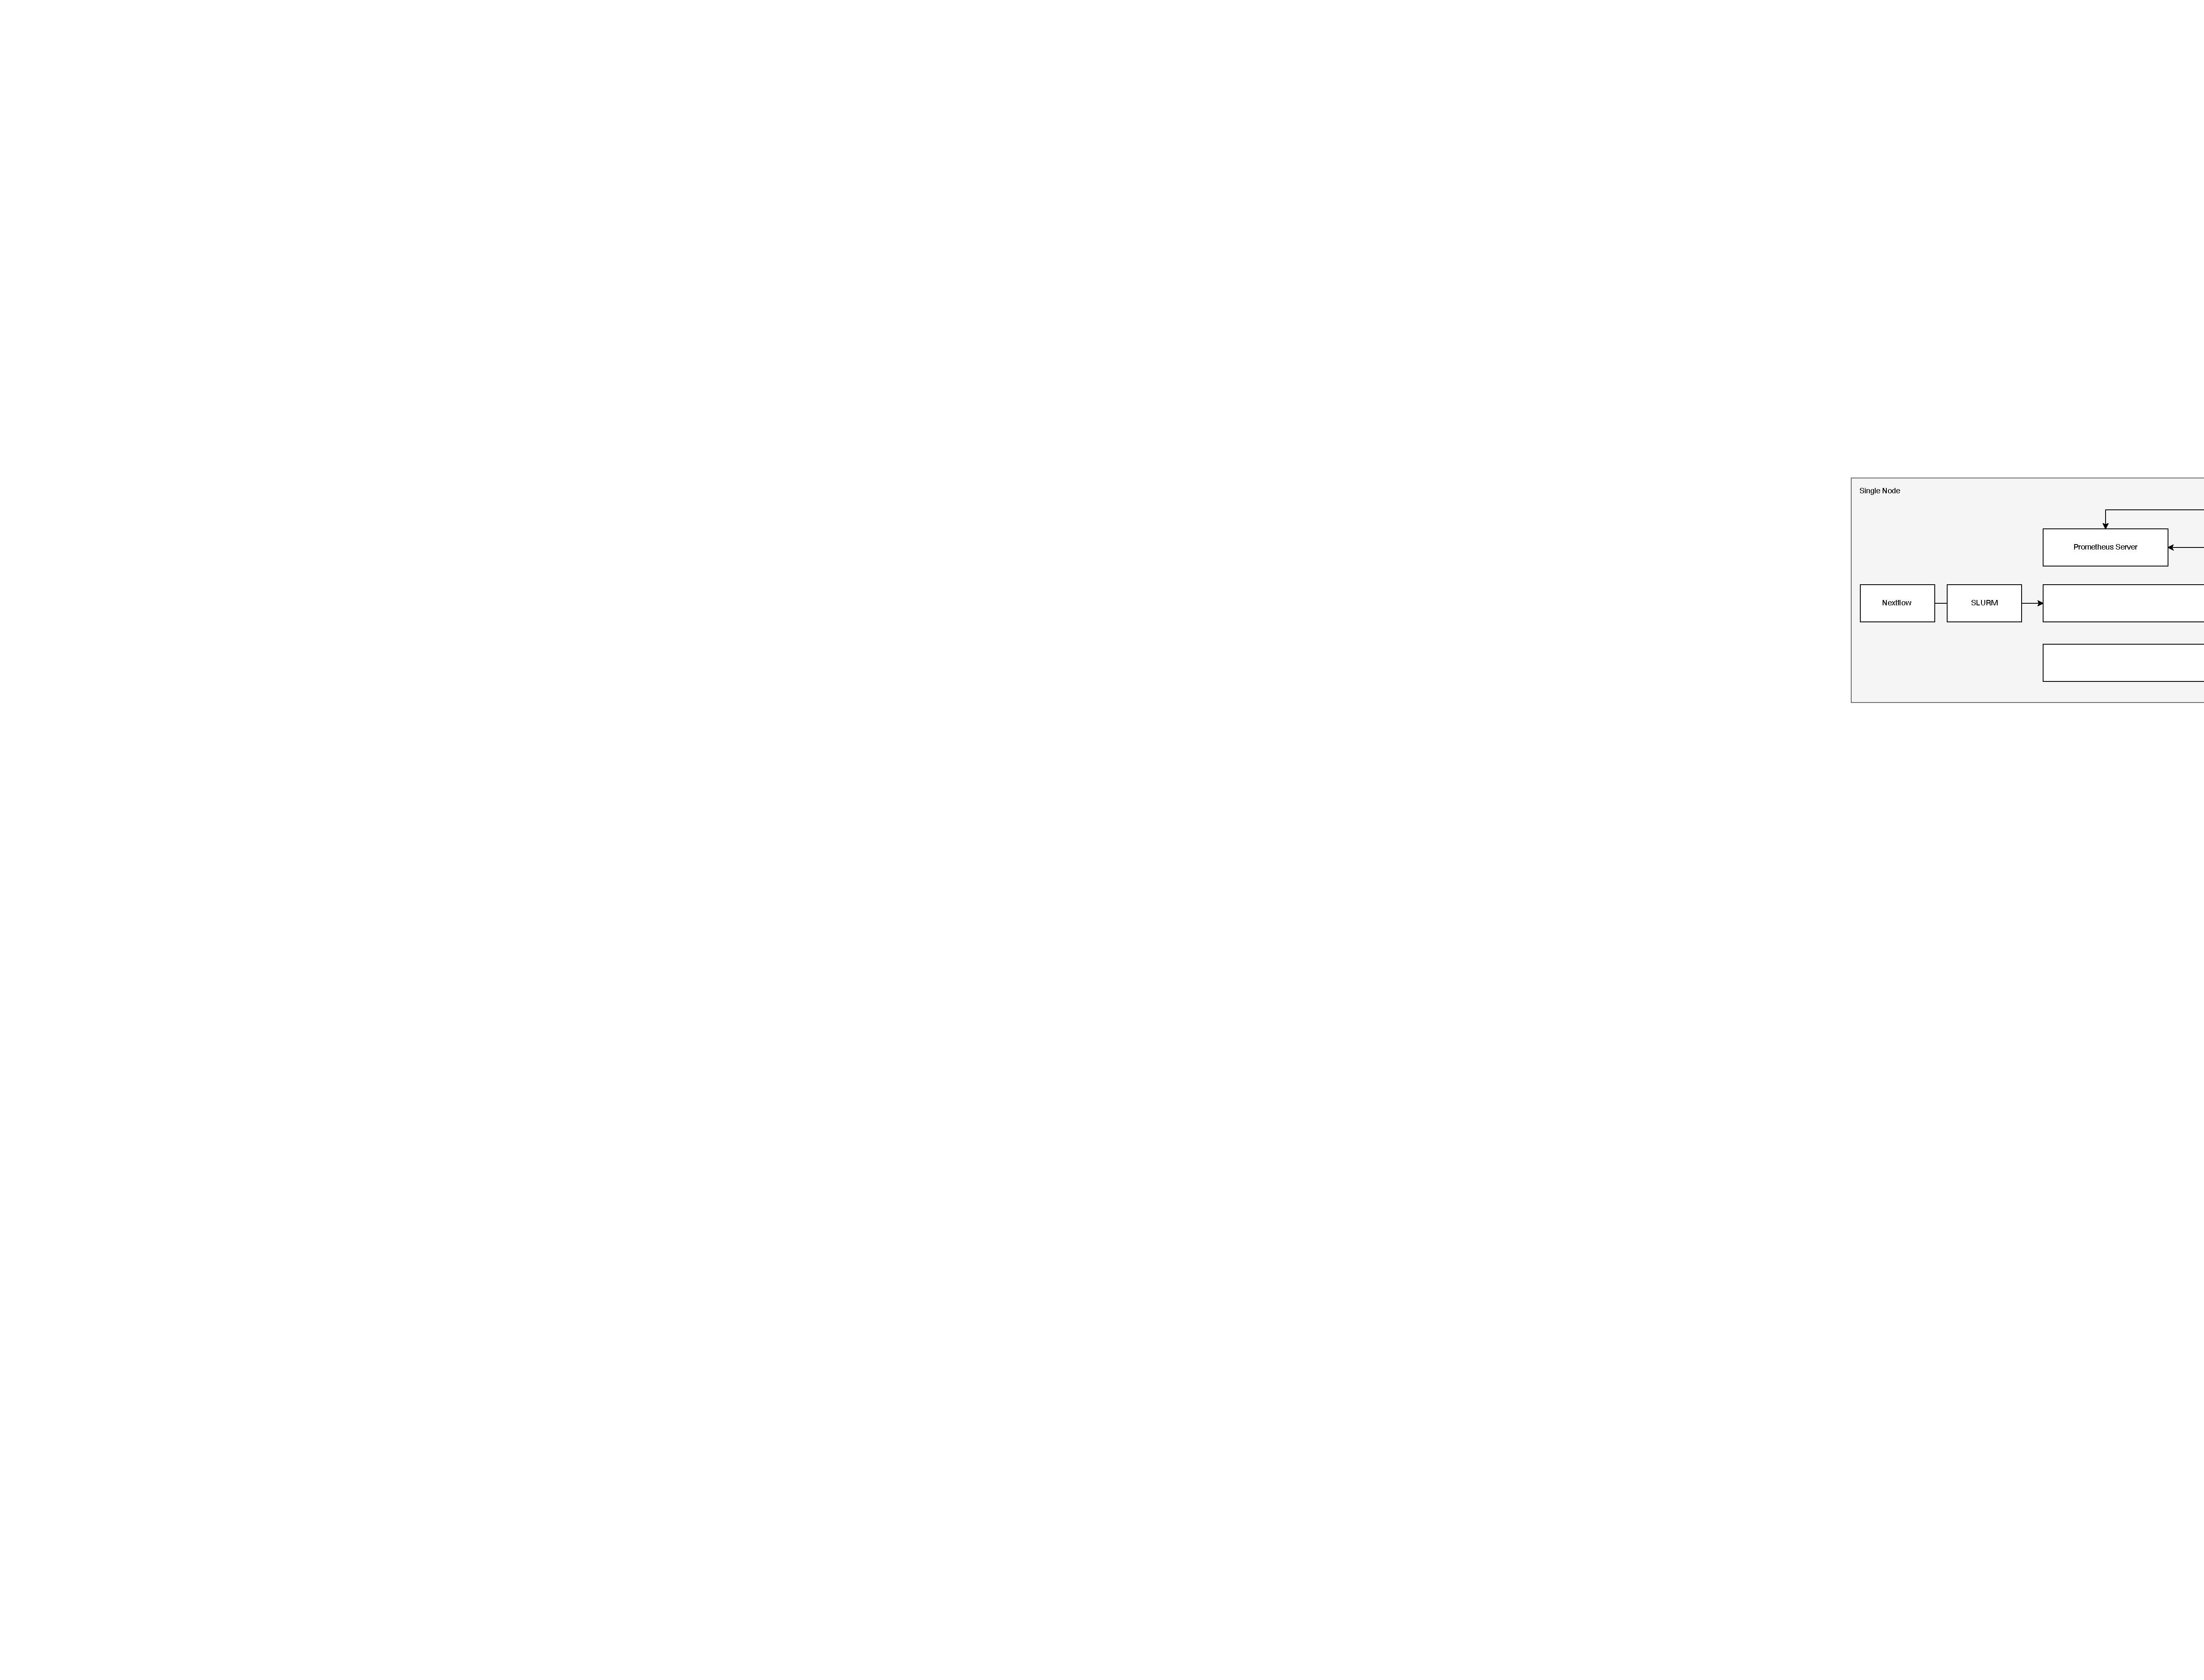
\includegraphics[width=\textwidth]{/home/nfomin3/dev/ThesisDocument/fig/04/04-monitoring.pdf} % Adjust the path if needed
    \caption{The monitoring client alongside the needed system components.}
    \label{fig:monitoring_client}
\end{figure}

The design of distributed HPC systems centers on three core aspects: resource allocation, queue ordering and dispatching, and job placement. To apply the concepts introduced in %\ref{sec:statistical_embedding_and_learning} and %\ref{sec:unsupervised_learning}, the simulation of scientific workflow task co-location adheres to these principles, providing a framework that supports multiple strategies for realistic exploration of this objective.
As seen in %\ref{fig:monitoring_client}, we structure the concept of the simulator around these three pillars.
The first pillar concerns resource allocation, which determines whether jobs are executed in exclusive or shared mode. Traditional HPC schedulers allocate full nodes to single jobs, task co-location naturally assumes that multiple tasks can coexist efficiently if they do not saturate the same resources simultaneously. The simulator therefore needs to model node-sharing policies where jobs may share cores or memory bandwidth.
Since the effectiveness of co-location depends on the characteristics of jobs and directly influence the throughput of the processing engine the simulator needs to offer an interface for alternative queue management strategies, ranging from conventional FIFO ordering to heuristic reordering that prioritizes beneficial pairings.
The third pillar, job placement, determines how tasks are assigned to available resources. The simulator needs to support random placement and heuristic strategies that intentionally group complementary tasks.
This setup aims at making it possible to study how the integration of task co-location choices during schedulung and task mapping influence overall system performance and resource efficiency, providing a controlled environment for algorithmic investigations.

\subsubsection{Heuristic Design}
\label{sec:heuristic_design}
Our algorithmic approach to define the behavior of the components resource manager, allocator and scheduler introduced in %\ref{fig:monitoring_client} is grounded in heuristic principles.
We choose to not formulate the embedding of co-location into the scheduling process as optimization problem but through decision-making within simple, interpretable scheduling and task mapping rules. Heuristic algorithms are well suited for such settings because they rely on deterministic, rule-based traversal of the search space rather than exhaustive or stochastic exploration. They exploit domain-specific knowledge, in our case energy-awareness and structured criteria—such as task priorities, resource affinities, or workload complementarities—to produce acceptable solutions efficiently without guaranteeing global optimality. We divide the task-to-node mapping into two steps. First, a queue of ready tasks is generated according to a defined orderign strategy before the mapping to resources of these ordered tasks is performed. For the scheduling we choose to adpot list-scheduling algorithms, which form one of the most established heuristic approaches for workflow scheduling. They assign a priority or ranking to each task based on topological and performance factors (e.g., critical path length, execution cost, or communication overhead), producing a priority list; second, they iteratively select the highest-priority unscheduled task and map it to a processor. As both phases can be modeled decoupled, there opens a chance to incorporate intelligent decision-making.
Machine learning list-scheduling approaches build on data-driven models that learn decision policies from historical workflow executions or directly during runtime. To complete the foundation of our heuristic design we formally introduce the simulation environment, consisting of the scientific workflow as the application that executes tasks and a system model that we use to represent our algorithmic approach to the co-location problem.

% System Model that was used for the heuristic design.

\textbf{Workflow Properties}

Let the workflow be represented as a directed acyclic graph (DAG)
\[
    G = (T, E)
\]
where
\begin{itemize}
    \item $T = \{t_1, t_2, \dots, t_n\}$ denotes the set of \textbf{tasks}, and
    \item $E \subseteq T \times T$ denotes \textbf{data or control dependencies} between tasks.
\end{itemize}
A directed edge $(t_i, t_j) \in E$ indicates that task $t_j$ can start only after $t_i$ has completed.

\textbf{Task Properties}

Each task \( t_i \in T \) is associated with the following attributes:
\[
    \begin{array}{rcll}
        \text{req\_cores}(t_i) & \in & \mathbb{N}_{\ge 1} & \text{number of CPU cores required}, \\[4pt]
        \text{req\_mem}(t_i)   & \in & \mathbb{R}_{>0}    & \text{memory requirement in bytes.}
    \end{array}
\]

\textbf{System Model}

Let \( \mathcal{H} = \{h_1, h_2, \dots, h_m\} \) denote the set of available \textbf{hosts},
where each host \( h_j \) is characterized by
\[
    C_j \in \mathbb{N}_{>0} \text{ (total number of cores)}, \qquad
    c(h_j) \in \mathbb{N}_{\ge 0} \text{ (current number of idle cores).}
\]

A \textbf{virtual machine (VM)} is represented as
\[
    v = (C_v, M_v, h_j),
\]
where \( C_v \) is the number of virtual cores, \( M_v \) the assigned memory,
and \( h_j \) the physical host on which it is instantiated.

The set of currently \textbf{ready tasks} (those whose dependencies are satisfied) is denoted by
\[
    \mathcal{Q} = \{t_1, t_2, \dots, t_k\}.
\]

\textbf{Host--Task Mapping}

A mapping of tasks to hosts and VMs is represented as
\[
    M = (h, \mathcal{T}_h, \text{colocMap}_h, \Phi_h),
\]
where
\begin{itemize}
    \item $h \in \mathcal{H}$ is the assigned host,
    \item $\mathcal{T}_h \subseteq T$ is the set of tasks mapped to $h$,
    \item $\text{colocMap}_h$ describes task clusters on $h$, and
    \item $\Phi_h$ represents associated file or data locations.
\end{itemize}
The set of mappings for an allocation interval is written as
\[
    \mathcal{M} = \{ M_1, M_2, \dots, M_p \}.
\]

\textbf{Task Co-location}

A \textbf{co-location mapping}, produced by a scheduler is defined as
\[
    \text{colocMap} = \{ (C_i, \mathcal{C}_i) \mid \mathcal{C}_i \subseteq T \},
\]
where $\mathcal{C}_i$ is a \textbf{cluster of tasks} to be executed together within a single virtual machine, ideally selected based on their resource affinity or complementary utilization patterns.



\textbf{Oversubscription}

An \textbf{oversubscription factor} $\alpha \in [0,1]$ allows up to
\[
    N_{\max}(h_j) = \lceil C_j (1 + \alpha) \rceil
\]
tasks to be scheduled concurrently on a VM on host $h_j$.


\textbf{Execution Dynamics}

At runtime:
\begin{itemize}
    \item \textbf{Node Assigners} determine host placement.
    \item \textbf{Schedulers} generate task queues and co-location groupings.
    \item \textbf{Allocators} instantiate and start VMs according to host-task mappings.
    \item The \textbf{Job Manager} executes tasks, monitors VM lifecycles, and updates resource states.
\end{itemize}

To evaluate the effectiveness of the proposed approach, we compare it against a series of progressively refined baseline algorithms that address the co-location problem with increasing complexity. These baselines range from simple scheduling heuristics to more advanced strategies that gradually incorporate awareness of co-location effects. The following table summarizes all baselines considered in this study. It is important to note that while some of them already involve concurrent execution of tasks, this represents uncontrolled co-location rather than informed or optimized placement. For clarity and conciseness, detailed algorithmic designs of these baselines are provided in the appendix, while this section focuses on describing their conceptual behavior.

% Blueprint Algorithm 
\paragraph{Baseline Algorithms}
\label{sec:baseline_algorithms}
% Overview table over all baselines
\begin{table}[H]
    \centering
    \caption{Overview of Baseline Scheduling Algorithms.}
    \label{tab:baseline_overview}
    \begin{tabularx}{\textwidth}{l l X}
        \toprule
        \textbf{Algorithm} & \textbf{Type}                                & \textbf{Description}                                                                                                          \\
        \midrule
        Baseline 1         & FIFO + Round-Robin                           & Executes tasks in FIFO order and assigns them to hosts in a round-robin fashion without co-location or backfilling.           \\

        Baseline 2         & FIFO + Backfilling                           & Assigns tasks in FIFO order to the first available host, allowing idle hosts to be backfilled opportunistically.              \\

        Baseline 3         & FIFO + VM Co-location                        & Groups multiple ready tasks on the same host within a single VM if sufficient resources are available.                        \\

        Baseline 3.1       & Max-Core VM Co-location                      & Prefers the host with the largest number of idle cores for task co-location to maximize utilization.                          \\

        Baseline 3.2       & Max-Parallel VM Co-location                  & Distributes ready tasks across all available hosts in parallel, promoting high concurrency across nodes.                      \\

        Baseline 4         & VM Co-location + Over-Subscription           & Extends co-location by allowing controlled CPU over-subscription on selected hosts using an oversubscription factor $\alpha$. \\

        Baseline 4.1       & Max-Parallel Co-location + Over-Subscription & Combines parallel host utilization with co-location and controlled CPU over-subscription for improved throughput.             \\
        \bottomrule
    \end{tabularx}
\end{table}

% W/O Co-location
% Baseline 1
The baseline scheduling algorithm implements a simple, sequential execution model designed to simulate isolated task processing within a virtualized cluster. The scheduling process is divided into three abstract components that operate in a fixed order: task scheduling, node assignment, and resource allocation. The scheduler applies a first-in, first-out (FIFO) policy, maintaining a queue of workflow tasks sorted by their readiness. Tasks are retrieved from this queue strictly in order of arrival, preserving dependency constraints and ensuring a fully deterministic execution sequence without reordering or prioritization.
Once a task is selected for execution, the node assignment component distributes it across available compute hosts using a round-robin policy. This mechanism cycles through hosts in sequence, ensuring an even and systematic distribution of tasks across the cluster. No host is assigned more than one active task at a time, enforcing exclusive execution and preventing contention for shared resources.

% Baseline 2
The next variant keeps the same FIFO scheduler and VM-based allocator as Baseline 1, but replaces exclusive node assignment with a greedy backfilling policy. Tasks are still dequeued strictly in arrival order by the FIFO scheduler. For each ready task, the node assignment component queries the cluster for the current number of idle cores per host and performs a first-fit scan: it selects the first host that reports at least one idle core, without requiring the host to be completely idle. The allocator then provisions a VM on the chosen host, binds the tasks inputs/outputs, submits the job to that VM, and on completion shuts the VM down and destroys it.
Conceptually, this turns the placement step into gap filling rather than strict exclusivity. Multiple tasks can be co-located on the same host up to its core capacity, increasing instantaneous parallelism and utilization.
% With co-location
% Baseline 3
Baseline 3 does not differ in the scheduling behavior but replaces the standard allocator and node assignment with components that allow for co-location. When the node assignment component queries the cluster for idle-core availability, it again selects the first host with available cores. However, instead of launching one VM per task, all ready tasks that fit within the hosts idle-core capacity are grouped into a single batch. These tasks are then co-located inside one shared VM instance that is dimensioned according to the aggregate resource requirements of the batch—its vCPU count and memory size are computed as the sum of the respective task demands.
Conceptually, this baseline captures the behavior of intra-VM co-location, where multiple independent tasks share the same virtual machine instead of being distributed across separate ones.
% Baseline 3.1
Baseline 3 is extended by 2 variants where the first one extends thenode assignment component to query the cluster for idle-core availability and selects the host with the maximum amount of available cores. However, instead of launching one VM per task, all ready tasks that fit within the hosts idle-core capacity are grouped into a single batch. These tasks are then co-located inside one shared VM instance that is dimensioned according to the aggregate resource requirements of the batch—its vCPU count and memory size are computed as the sum of the respective task demands.
% Baseline 3.2
The second extension replaces the placement policy with a selection step for the host with maximum idle cores. At each dispatch, the node-assignment component queries the cluster for the current idle cores per host map and picks the host with the largest number of free cores. It then forms a batch by taking as many ready tasks from the FIFO head as the chosen host can accommodate. Compared to first-fit co-location, it tends to reduce residual fragmentation by packing work onto the most spacious node, while still honoring FIFO ordering and leaving task runtime/I/O handling unchanged.
% Baseline 4
The 4th baseline retains the same FIFO scheduler but introduces a node assignment and allocation policy focused on maximizing parallel host utilization. Upon each scheduling cycle, the node assignment component queries the cluster for the current number of idle cores per host, filters out fully occupied nodes, and ranks the remaining hosts in descending order of available cores. It then assigns tasks in batches, filling the host with the highest idle capacity first and grouping as many ready tasks as the hosts idle-core count allows. Once the first host is filled, the process continues with the next host until all tasks in the ready queue are mapped.
The allocator provisions one VM per host batch, sizing it to match the aggregate requirements of all tasks assigned to that host. The resulting VMs vCPU and memory configuration reflect the total core and memory demands of the batch. Each task in the batch is submitted as an independent job to the same virtual compute service, and the VM remains active until all its co-located tasks have finished, at which point it is shut down and destroyed.
% Baseline 4.1
% The last baseline extends the previous one by allowing controlled CPU over-subscription during co-location.
% At each scheduling cycle, the node assignment component queries per-host idle cores, sorts hosts in descending idle capacity, and fills the largest host first. Unlike the non-oversubscribed version, the per-host batch may exceed the currently idle cores by a fixed factor (e.g., 25\%): the batch limit is set to \lceil idle\_cores \times (1 + oversub\_factor) \rceil. The procedure continues down the ranked host list, forming one batch per host in the same cycle.
The allocator provisions one VM per host batch, but caps the VMs vCPU count to the hosts actual idle cores at allocation time (not the sum of task core demands), while sizing memory to the aggregate of the batched tasks. All tasks in the batch are then submitted to that single VM and execute concurrently on a vCPU pool intentionally smaller than their combined declared cores. The VM remains active until all co-located tasks complete, then it is shut down and destroyed.
Crucially, the degree of contention—and thus realized speedup or slowdown—depends on the complementarity of the co-located task profiles. When CPU-, memory-, and I/O-intensive phases overlap unfavorably oversubscription amplifies interference and queueing on scarce vCPUs. When profiles are complementary, the same oversubscription admits more useful overlap with less contention, improving per-host throughput. Conceptually, this variant implements parallel, capacity-ranked co-location with controlled oversubscription.

\paragraph{Contention-aware Co-location strategies}
\label{sec:co-location_strategies}


% Table with ShaRiff Overview stuff.
\begin{table}[H]
    \centering
    \caption{Overview of ShaRiff and ShaReComp Scheduling Algorithms.}
    \label{tab:shariff_overview}
    \begin{tabularx}{\textwidth}{l l X}
        \toprule
        \textbf{Algorithm} & \textbf{Type}                                         & \textbf{Description}                                                                                                                         \\
        \midrule
        ShaRiff 1          & Contention-Aware Co-location                          & Uses the ShaReComp API to determine affinity-based co-location groups, minimizing interference between tasks.                                \\

        ShaRiff 2          & Adaptive Co-location + Over-Subscription              & Extends ShaRiff 1 by allowing safe CPU over-subscription based on affinity predictions.                                                      \\

        ShaRiff 3          & Round-Robin Node Assignment + Co-location             & Schedules tasks round-robin across hosts while applying affinity-based co-location through the ShaReComp API.                                \\

        ShaReComp          & Adaptive Max-Parallel Co-location + Over-Subscription & Integrates parallel scheduling, affinity-based co-location, and controlled over-subscription for optimized throughput and energy efficiency. \\
        \bottomrule
    \end{tabularx}
\end{table}

% Explain and visualize ShaRiff in it's variants algorihtmically and algorihtms after each paragraph.
% ShaRiff 1

% Algorithm
\begin{algorithm}[H]
    \caption{ShaRiff 1 — Contention-aware Max-Parallel VM Co-Location Scheduling}
    \label{alg:sharecomp}
    \KwIn{workflow \( G=(T,E) \), hosts \( \mathcal{H}=\{h_1,\dots,h_m\} \), idle cores \( c(h_j) \), ShaReComp co-location API \( \mathcal{S} \)}
    \KwOut{all tasks \( t_i\in T \) executed with contention-aware co-location for improved efficiency and utilization}

    \BlankLine
    Initialize idle cores \( c(h_j)\gets C_j \) for all \( h_j\in\mathcal{H} \);
    Initialize ready queue \( \mathcal{Q} \) with all source tasks of \( G \) (FIFO order)

    \BlankLine
    \While{not all tasks \( t_i\in T \) completed}{
        \If{\( \mathcal{Q} \) is empty}{
            Wait until any task \( t_r \) completes;
            Release its cores: \( c(h(t_r)) \gets c(h(t_r)) + \text{req\_cores}(t_r) \);
            For each successor \( t_s \) of \( t_r \), enqueue \( t_s \) into \( \mathcal{Q} \) if all predecessors are completed;
            \textbf{continue}
        }

        Build available-host list \( L=\{\,h\in\mathcal{H}\mid c(h)>0\,\} \), sorted by \( c(h) \) descending;
        Initialize empty host task mapping list \( \mathcal{M} \);

        \BlankLine
        \ForEach{host \( h\in L \) and while \( \mathcal{Q} \) not empty}{
            Select up to \( c(h) \) ready tasks from \( \mathcal{Q} \) into \( \mathcal{T}_h \);
            Compute file-location map \( \Phi(\mathcal{T}_h) \);
            Query ShaReComp API: \( \text{colocMap} \gets \mathcal{S}(\mathcal{T}_h) \) \tcp*[r]{returns co-location groups}
            Add mapping \( (h,\mathcal{T}_h,\Phi(\mathcal{T}_h),\text{colocMap}) \) to \( \mathcal{M} \);
        }

        \BlankLine
        \ForEach{mapping \( (h,\mathcal{T}_h,\Phi,\text{colocMap}) \in \mathcal{M} \)}{
            \ForEach{group \( \mathcal{C}_k \in \text{colocMap} \)}{
                \( C_{\text{req}} \gets \text{sum(req\_cores}(\mathcal{C}_k)) \);
                \( M_{\text{req}} \gets \text{sum(req\_mem}(\mathcal{C}_k)) \);
                Allocate \( v_h = (C_{\text{req}}, M_{\text{req}}, h) \);
                Launch all \( t \in \mathcal{C}_k \) on \( v_h \);
                \( c(h) \gets \max(0, c(h) - C_{\text{req}}) \);
                Remove \( \mathcal{C}_k \) from \( \mathcal{Q} \);
            }
        }

        \BlankLine
        Wait until any task \( t_r \) completes;
        Release its cores: \( c(h(t_r)) \gets c(h(t_r)) + \text{req\_cores}(t_r) \);
        \If{no active tasks remain on its VM}{ Destroy VM }
        For each successor \( t_s \) of \( t_r \): if all predecessors are completed, enqueue \( t_s \) into \( \mathcal{Q} \);
    }
    \Return{workflow complete}

\end{algorithm}
This variant implements ShaRiff (share resources if feasible), which augments the FIFO pipeline with an external co-location adviser and a cluster-aware allocator. Tasks are still dequeued in strict arrival order. Before placement, the scheduler invokes ShaRiff with the current set of ready tasks and receives clusters of jobs that are predicted to co-locate well (i.e., complementary resource profiles / low expected interference). The node-assignment stage then ranks hosts by descending idle-core capacity and fills the largest host first: it forms a batch of up to that hosts idle cores and attaches the ShaRiff cluster map to the batch; if tasks remain, it proceeds to the next host in the ranked list. A small-queue fast path ensures dispatch even when only a few tasks are available.
The allocator realizes the advisers plan one VM per recommended cluster on the chosen host. For each multi-task cluster, it provisions a VM whose vCPU count and memory equal the sum of the clustered tasks declared requirements, starts the VM, and submits the tasks to that same virtual compute service. Singleton clusters are grouped into a shared VM on the host (current variant) to avoid VM fragmentation; each submitted task keeps its own job identity, and the allocator tracks VM lifecycle across all tasks assigned to it, tearing the VM down only after the last co-located task completes.
Conceptually, ShaRiff preserves FIFO ordering and capacity-ranked host filling, but replaces random batching with adviser-driven clustering. The effect is to co-locate tasks that are likely complementary (e.g., CPU-bound with I/O-bound), thereby reducing contention and improving per-host utilization without oversubscription. When the adviser yields singletons, the system still shares if feasible by pooling them into a shared VM, maintaining the same deterministic provisioning and lifecycle rules.

% ShaRiff 2

% Algorithm
\begin{algorithm}[H]
    \caption{ShaRiff 2 — Adaptive Max-Parallel VM Co-Location with Controlled Over-Subscription}
    \label{alg:sharecomp_oversub}
    \KwIn{workflow \( G=(T,E) \), hosts \( \mathcal{H}=\{h_1,\dots,h_m\} \), idle cores \( c(h_j) \), oversubscription factor \( \alpha \), ShaReComp co-location API \( \mathcal{S} \)}
    \KwOut{workflow executed with affinity-based co-location, maximal host parallelism, and safe oversubscription}

    \BlankLine
    Initialize idle cores \( c(h_j)\gets C_j \) for all \( h_j\in\mathcal{H} \)
    Initialize ready queue \( \mathcal{Q} \) with all source tasks of \( G \) (FIFO order)

    \BlankLine
    \While{not all tasks \( t_i\in T \) completed}{
        \If{\( \mathcal{Q} \) is empty}{
            Wait until any task \( t_r \) completes
            Release its cores: \( c(h(t_r)) \gets c(h(t_r)) + \text{req\_cores}(t_r) \)
            For each successor \( t_s \) of \( t_r \), enqueue \( t_s \) into \( \mathcal{Q} \) if all predecessors are completed\\
            \textbf{continue}
        }

        Build available-host list \( L=\{\,h\in\mathcal{H}\mid c(h)>0\,\} \), sorted by \( c(h) \) descending
        Initialize empty host task mapping list \( \mathcal{M} \)

        \BlankLine
        \ForEach{host \( h\in L \) and while \( \mathcal{Q} \) not empty}{
            Compute oversubscription limit \( n_{\max} = \lceil c(h) \times (1 + \alpha) \rceil \)
            Select up to \( n_{\max} \) ready tasks from \( \mathcal{Q} \) into \( \mathcal{T}_h \)
            Compute file-location map \( \Phi(\mathcal{T}_h) \)
            Query ShaReComp API: \( \text{colocMap} \gets \mathcal{S}(\mathcal{T}_h) \) \tcp*[r]{returns co-location groups}
            Add mapping \( (h,\mathcal{T}_h,\Phi(\mathcal{T}_h),\text{colocMap}) \) to \( \mathcal{M} \)
        }

        \BlankLine
        \ForEach{mapping \( (h,\mathcal{T}_h,\Phi,\text{colocMap}) \in \mathcal{M} \)}{
            \ForEach{group \( \mathcal{C}_k \in \text{colocMap} \)}{
                \( C_{\text{req}} \gets \text{sum(req\_cores}(\mathcal{C}_k)) \)
                \( M_{\text{req}} \gets \text{sum(req\_mem}(\mathcal{C}_k)) \)
                \If{\( C_{\text{req}} > c(h) \)}{
                    Allocate \( v_h = (c(h), M_{\text{req}}, h) \); \tcp*[r]{oversubscription active}
                }
                \Else{
                    Allocate \( v_h = (C_{\text{req}}, M_{\text{req}}, h) \)
                }
                Launch all \( t \in \mathcal{C}_k \) on \( v_h \)
                \( c(h) \gets \max(0, c(h) - C_{\text{req}}) \)
                Remove \( \mathcal{C}_k \) from \( \mathcal{Q} \)
            }
        }

        \BlankLine
        Wait until any task \( t_r \) completes
        Release its cores: \( c(h(t_r)) \gets c(h(t_r)) + \text{req\_cores}(t_r) \)
        \If{no active tasks remain on its VM}{ Destroy VM }
        For each successor \( t_s \) of \( t_r \): if all predecessors are completed, enqueue \( t_s \) into \( \mathcal{Q} \)
    }
    \Return{workflow complete}
\end{algorithm}

This variant retains the ShaRiff-augmented FIFO pipeline but enables controlled oversubscription during placement and VM sizing. Tasks are dequeued in arrival order. Before dispatch, the scheduler queries ShaRiff with the current ready set and receives clusters of tasks predicted to co-locate well (complementary resource use / low interference). Hosts are ranked by descending idle-core capacity; the assigner then fills the largest host first with a batch whose size may exceed the hosts free cores by a fixed factor (e.g., +25\%). If tasks remain, it proceeds to the next host and repeats.
The allocator implements the advisers plan one VM per cluster on the chosen host, but with oversubscription semantics. For multi-task clusters, it provisions a VM whose vCPU and memory equal the sum of the clusters requests—even if that exceeds the hosts currently free cores (hard oversub). For singleton clusters collected on the same host, it provisions a shared VM and caps vCPUs at the hosts free cores when necessary (soft cap). In both cases the VM is started once, all tasks in the cluster are submitted to the same virtual compute service, and the VM is torn down only after the last co-located task finishes.
Conceptually, this policy combines adviser-driven co-location with capacity-aware overbooking: FIFO ordering and capacity-ranked host filling are preserved, but batches may intentionally outsize instantaneous capacity to exploit latency hiding and temporal slack (e.g., I/O wait, imbalanced phases). Because ShaRiff groups complementary tasks, oversubscription tends to translate into higher throughput and energy efficiency than naive overbooking; however, when clustered tasks are less complementary, contention can surface, making this variant an explicit trade-off between utilization and interference.

% ShaRiff 3

% Algorithm

\begin{algorithm}[H]
    \caption{ShaRiff 3 — Round-Robin Node Assignment with contention-aware VM Co-Location}
    \label{alg:sharecomp_rr}
    \KwIn{workflow \( G=(T,E) \), hosts \( \mathcal{H}=\{h_1,\dots,h_m\} \), idle cores \( c(h_j) \), ShaReComp co-location API \( \mathcal{S} \)}
    \KwOut{tasks executed using round-robin host selection with affinity-based VM co-location}

    \BlankLine
    Initialize idle cores \( c(h_j)\gets C_j \) for all \( h_j\in\mathcal{H} \)
    Initialize ready queue \( \mathcal{Q} \) with all source tasks of \( G \) (FIFO order)
    Initialize round-robin index \( r \gets 0 \)

    \BlankLine
    \While{not all tasks \( t_i\in T \) completed}{
        \If{\( \mathcal{Q} \) is empty}{
            Wait until any task \( t_r \) completes
            Release its cores: \( c(h(t_r)) \gets c(h(t_r)) + \text{req\_cores}(t_r) \)
            For each successor \( t_s \) of \( t_r \), enqueue \( t_s \) into \( \mathcal{Q} \) if all predecessors are completed\\
            \textbf{continue}
        }

        Select next host \( h = \mathcal{H}[r \bmod |\mathcal{H}|] \)
        Update round-robin index: \( r \gets (r + 1) \bmod |\mathcal{H}| \)
        Retrieve available cores \( C = c(h) \)
        Select up to \( C \) ready tasks from \( \mathcal{Q} \) into \( \mathcal{T}_h \)
        Query ShaReComp API: \( \text{colocMap} \gets \mathcal{S}(\mathcal{T}_h) \) \tcp*[r]{returns co-location groups}

        \BlankLine
        \ForEach{group \( \mathcal{C}_k \in \text{colocMap} \)}{
            \( C_{\text{req}} \gets \text{sum(req\_cores}(\mathcal{C}_k)) \)
            \( M_{\text{req}} \gets \text{sum(req\_mem}(\mathcal{C}_k)) \)
            Allocate \( v_h = (C_{\text{req}}, M_{\text{req}}, h) \)
            Launch all \( t \in \mathcal{C}_k \) on \( v_h \)
            \( c(h) \gets \max(0, c(h) - C_{\text{req}}) \)
            Remove \( \mathcal{C}_k \) from \( \mathcal{Q} \)
        }

        \BlankLine
        Wait until any task \( t_r \) completes
        Release its cores: \( c(h(t_r)) \gets c(h(t_r)) + \text{req\_cores}(t_r) \)
        \If{no active tasks remain on its VM}{ Destroy VM }
        For each successor \( t_s \) of \( t_r \): if all predecessors are completed, enqueue \( t_s \) into \( \mathcal{Q} \)
    }
    \Return{workflow complete}
\end{algorithm}

This variant preserves FIFO dequeuing but combines round-robin first-fit placement with ShaRiff-guided intra-VM co-location. The scheduler releases tasks strictly in arrival order. The node-assignment component scans hosts in round-robin/first-fit fashion and picks the first host reporting at least one idle core. It then pulls up to that hosts idle-core capacity worth of ready tasks and queries ShaRiff for a co-location plan over this batch.
The allocator realizes ShaRiffs plan one VM per suggested cluster on the chosen host. For each multi-task cluster, it sizes the VM by summing vCPU and memory requirements of the clusters tasks, starts the VM, and submits all cluster tasks to the same virtual compute service. Tasks that ShaRiff leaves as singletons are grouped onto an additional shared VM on that host; its size is the aggregate of the singletons requests. VM lifecycle is managed per cluster: each VM stays up until all of its assigned tasks complete, then is shut down and destroyed.
Conceptually, the policy is first-fit host, adviser-driven packing. It preserves FIFO ordering and simple first-fit host selection while letting ShaRiff decide which tasks should share a VM to reduce interference (by favoring complementary profiles). Unlike the max-parallel variants, this strategy does not oversubscribe cores; it fills only the currently free capacity of the first eligible host and relies on ShaRiffs clustering to raise utilization and efficiency through informed co-location.

% TODO: This part needs to be reworked.
% MinMin extension
This scheduler extension augments the ShaRiff-based variants with a MinMin ordering layer, a classical heuristic from list scheduling. In standard list scheduling, tasks are iteratively selected based on their earliest estimated completion time; Min Min specifically chooses, at each step, the task (or cluster) with the minimum predicted runtime among all ready candidates and schedules it first. Here, this principle is applied not to individual tasks but to task clusters produced by ShaRiffs co-location analysis.
For each scheduling interval, the scheduler requests from ShaRiff a co-location partition of the ready tasks, grouping them into clusters that are predicted to interact efficiently when sharing a VM. It then queries a prediction service for each cluster, obtaining runtime estimates through the chosen model (e.g., KCCA). The clusters are ordered by ascending predicted runtime, and this order defines the execution sequence. Node selection and VM provisioning are delegated to the ShaRiff node assignment and allocator components, which handle placement and resource sizing as usual.
Conceptually, this forms a Min Min list scheduler over co-located clusters: it maintains ShaRiffs intelligent co-location strategy while globally minimizing queueing delay and improving average completion time by prioritizing faster clusters. This layer is independent of the underlying allocation or node assignment logic and purely refines execution ordering to exploit performance prediction while preserving all structural and capacity constraints of the ShaRiff framework.